\section{Experimental Details}\label{app:details}

\paragraph{Base SAE training.} Each of the 108 base SAEs was trained in one uninterrupted run of 15{,}000 Adam steps
(learning rate $3\times10^{-4}$, batch 256 sampled with replacement, gradient clipping at 10), about 3.84M samples or 38
passes over the 101{,}600 OWT training tokens. A multiplicative controller adjusted the sparsity coefficient every 25
steps towards L0 = 128 for ReLU and JumpReLU; TopK fixes L0 by construction. Decoder columns were renormalised to unit
norm after every step. An earlier version of the layers mixed optimiser procedures; all 108 SAEs were retrained with the
uniform protocol, which changed explained variance by at most 0.006 and no ranking.

\paragraph{Fine-tuning (Method A, output-KL, IMP-L).} Every fine-tune starts from a trained base SAE and runs 500 Adam
steps at learning rate $10^{-5}$, with the sparsity controller continued from the base coefficient. Method A trains on
reconstruction of GoT group-A statements with OWT replay; the OWT-only control continues on OWT alone; output-KL adds a
KL term between the original and spliced next-token distributions. A cell's criterion is met when the arm is better on
all three seeds and the mean paired difference exceeds twice its standard deviation. Guards: OWT L0 within $\pm5\,\%$ of
the base, OWT explained variance at most 0.005 below the base (output-KL: 0.02 below Method A), spliced $\Delta$CE at most
$1.10\times$ the base, and no loss of the GoT truth preference beyond 0.018. Layer-6 results, the per-layer
classifications and all paired differences are in Tables~\ref{tab:ft6}--\ref{tab:impl9}.

\paragraph{Data-scaled SAEs (R2) and KL fine-tune (R4).} R2 SAEs were trained on activations streamed from GPT-2 into
a GPU buffer, with the encoder initialised to the decoder transpose, input scaling folded into the weights and cosine
learning-rate decay; 39 SAEs were trained in 5.5 hours on one NVIDIA A10G. A comparison is an improvement only if all
nine new/old seed pairs favour the new SAE and the Welch 95\,\% interval excludes zero; every R2 SAE had OWT L0 within
$\pm10\,\%$ of 128. R4 fine-tunes the R2 TopK-12288 SAEs at layers 8 and 11 for 5M tokens at learning rate
$2\times10^{-5}$ with NMSE plus $\alpha\,\mathrm{KL}(p_{\text{orig}}\|p_{\text{spliced}})$, with $\alpha$ set by first-batch
scale matching, against an MSE-only control on identical tokens.

\paragraph{Causal decomposition.} At a site, $\Delta=x_H-x_U$, $\Delta_{\text{rec}}=\hat{x}_H-\hat{x}_U$ and
$\Delta_{\text{err}}=e_H-e_U$, so $\Delta=\Delta_{\text{rec}}+\Delta_{\text{err}}$ exactly. Shapley shares are
$\phi_{\text{rec}}=(T_{\text{rec}}+T_{\text{full}}-T_{\text{err}})/2$; they are not interpreted additively when the
interaction is large. All exact checks pass ($\Delta$ identity error $9.5\times10^{-7}$; $T_{\text{full}}$ reproduces
M3 to $7\times10^{-8}$). Each patch adds a vector to the dishonest run's original activation; it is not a full splice.

\section{Dataset Splits, Leakage Controls and Test Exposure}\label{app:exposure}

OWT is split by document and GoT by city, so no document or city appears in two splits. Training objectives may use GoT
group A only, and independent evaluation probes are fitted on group B; an audit of an earlier objective whose teacher
was also the evaluation probe is described in Section~\ref{sec:finetune}. RepE-LM pairs differ in one token at a fixed
position, every tested shortcut has AUROC 0.50, and the 14 validation statements with an opposite-label near duplicate in
training change any reported gap by at most 0.02. The Gemma evaluation and reference documents are disjoint by
construction, the mean-ablation vector uses the reference set only, and the Pile test file was never read.

Test exposure is as follows. The OWT test split was used for the reconstruction table and once more in the
pre-registered M5 pass. The GoT test split was scored for all 108 base SAEs with frozen probes and twice for historical
layer-6 fine-tunes before M5, so it is treated as previously exposed. The RepE-LM test split has a frozen protocol but
no reported result. M0--M4, IMP-L, RLM-RP, E3, R5, E2, PCA-CM and M6 used no test rows.

\section{SAE Architectures and Layer Conventions}\label{app:arch}

GPT-2 SAEs (in-house and \texttt{gpt2-small-res-jb}) read \texttt{blocks.$L$.hook\_resid\_pre}, the input to block $L$.
Gemma Scope SAEs read \texttt{blocks.$L$.hook\_resid\_post}, the output of layer $L$, which in the Hugging Face
implementation equals \texttt{hidden\_states[$L$+1]}; this equality was checked exactly for every document. The two
conventions belong to the SAE families and are not a mapping between models. The in-house SAE forward pass is given in
Section~\ref{sec:saes}; the Gemma Scope forward pass is
$f=\mathrm{JumpReLU}_\theta(W_{\text{enc}}x+b_{\text{enc}})$, $\hat{x}=W_{\text{dec}}f+b_{\text{dec}}$, computed in fp32 on bf16
activations, as released.

\section{Additional GPT-2 Results}\label{app:gpt2}

This appendix collects the detailed tables and secondary figures behind Sections~\ref{sec:beyond}
and~\ref{sec:improve}. All are \evlabel{validation} findings unless their caption says otherwise.

% generated by scripts/shared/build_paper_artifacts.py from results/openwebtext/spliced_evaluation/summary.csv
\begin{table}[t]
\centering
\small
\caption{Behavioural faithfulness: GPT-2 with the SAE reconstruction spliced in at every non-BOS position (OWT validation; original CE 3.396 nats/token; matched seeds only). Source: \texttt{results/openwebtext/spliced\_evaluation/summary.csv}.}
\label{tab:splice}
\begin{adjustbox}{max width=\linewidth}
\begin{tabular}{rcccccc}
\toprule
Layer & \multicolumn{3}{c}{Spliced $\Delta$CE (nats/token, $\downarrow$)} & \multicolumn{3}{c}{Loss recovered ($\uparrow$)} \\
\cmidrule(lr){2-4}\cmidrule(lr){5-7}
 & ReLU & TopK & JumpReLU & ReLU & TopK & JumpReLU \\
\midrule
0 & 0.029 & 0.057 & 0.036 & 0.996 & 0.991 & 0.995 \\
1 & 0.019 & 0.026 & 0.009 & 0.998 & 0.997 & 0.999 \\
2 & 0.037 & 0.038 & 0.021 & 0.995 & 0.994 & 0.997 \\
3 & 0.078 & 0.057 & 0.040 & 0.987 & 0.991 & 0.994 \\
4 & 0.114 & 0.075 & 0.058 & 0.984 & 0.990 & 0.992 \\
5 & 0.167 & 0.105 & 0.091 & 0.967 & 0.980 & 0.982 \\
6 & 0.177 & 0.104 & 0.092 & 0.966 & 0.980 & 0.982 \\
7 & 0.198 & 0.114 & 0.106 & 0.963 & 0.979 & 0.980 \\
8 & 0.223 & 0.126 & 0.117 & 0.958 & 0.976 & 0.978 \\
9 & 0.250 & 0.150 & 0.140 & 0.951 & 0.971 & 0.973 \\
10 & 0.280 & 0.168 & 0.164 & 0.947 & 0.968 & 0.969 \\
11 & 0.358 & 0.213 & 0.225 & 0.930 & 0.958 & 0.956 \\
\bottomrule
\end{tabular}
\end{adjustbox}
\end{table}

% generated by scripts/shared/build_paper_artifacts.py from results/repe/repe_lm_gates/gates.json
\begin{table}[t]
\centering
\small
\caption{M1 RepE-LM construction and gates (pre-registered pass rules). Source: \texttt{results/repe/repe\_lm\_gates/gates.json}.}
\label{tab:m1}
\begin{adjustbox}{max width=\linewidth}
\begin{tabular}{llp{0.62\linewidth}}
\toprule
Gate & Status & Evidence (train statements) \\
\midrule
K1 construction & PASS & 6,072 pairs; max residual difference before the swapped token 0.0 at all 12 layers \\
K2 shortcuts & PASS & max deviation of any shortcut AUROC from 0.5: 5.6e-17 \\
K3 positive control & PASS & unmasked bag-of-words AUROC 1.000 \\
K5 persona meaning & PASS & leave-one-pair-out AUROC 0.701 at layer 8 (CI low 0.689); passing layers [8, 11] \\
K6 leakage & PASS & 0 exact overlaps; 0 same-label near-duplicates \\
K7 behaviour & PASS & median KL(H$\|$U) 0.0186 vs KL(H$\|$H$^\prime$) 0.0092 nats; ratio 1.99; Wilcoxon $p=3e-68$ \\
\bottomrule
\end{tabular}
\end{adjustbox}
\end{table}

% generated by scripts/shared/build_paper_artifacts.py from results/repe/repe_lm_representation_preservation/summary_by_layer_arch.csv, results/repe/repe_lm_representation_preservation/original_by_layer.csv
\begin{table}[t]
\centering
\small
\caption{RLM-RP: RepE-LM persona preservation by layer for the 99 base SAEs at layers 1--11 (VALIDATION; final token; mean$\pm$sd over 3 seeds where shown). ``Orig.'': frozen logistic AUROC on original activations. Gaps are original $-$ reconstructed AUROC ($\downarrow$). ``Noise'': frozen gap under isotropic noise with the SAE error's norm. Held-out: frozen persona probe on never-fitted templates T5/T6. $\Delta=x_H-x_U$ per pair; EV and L0 on all RepE-LM validation prompts (L0 matched on OWT, not here). Layer 0 is excluded: AUROC is 0.5 by construction. Source: \texttt{results/\allowbreak{}repe/\allowbreak{}repe\_lm\_representation\_preservation/\allowbreak{}summary\_by\_layer\_arch.csv}; \texttt{results/\allowbreak{}repe/\allowbreak{}repe\_lm\_representation\_preservation/\allowbreak{}original\_by\_layer.csv}.}
\label{tab:rlm_layers}
\begin{adjustbox}{max width=\linewidth}
\begin{tabular}{llcccccccccccc}
\toprule
L & Orig. & SAE & Frozen log. gap & Noise & Frozen m.-m. & Re-trained gap & Held-out T5/T6 & Neutral re-tr. & $\cos(\Delta,\hat\Delta)$ & $\|\hat\Delta\|/\|\Delta\|$ & m.-m. cos & EV & L0 \\
\midrule
1 & 0.657 & ReLU & 0.113$\pm$0.002 & 0.033 & 0.035 & 0.095$\pm$0.006 & 0.026 & 0.085 & 0.52 & 0.69 & 0.74 & 0.896 & 214 \\
 &  & TopK & 0.095$\pm$0.003 & 0.037 & 0.029 & 0.083$\pm$0.012 & 0.026 & 0.085 & 0.37 & 1.46 & 0.73 & 0.857 & 128 \\
 &  & JumpReLU & 0.109$\pm$0.003 & 0.035 & 0.027 & 0.097$\pm$0.004 & 0.028 & 0.082 & 0.38 & 1.31 & 0.74 & 0.909 & 208 \\
\midrule
2 & 0.728 & ReLU & 0.156$\pm$0.004 & 0.054 & 0.055 & 0.144$\pm$0.005 & 0.066 & 0.072 & 0.58 & 0.69 & 0.77 & 0.898 & 201 \\
 &  & TopK & 0.151$\pm$0.006 & 0.060 & 0.055 & 0.137$\pm$0.007 & 0.060 & 0.080 & 0.40 & 1.33 & 0.70 & 0.874 & 128 \\
 &  & JumpReLU & 0.143$\pm$0.008 & 0.049 & 0.046 & 0.122$\pm$0.009 & 0.060 & 0.073 & 0.43 & 1.33 & 0.74 & 0.915 & 207 \\
\midrule
3 & 0.780 & ReLU & 0.185$\pm$0.006 & 0.073 & 0.082 & 0.170$\pm$0.006 & 0.087 & 0.064 & 0.56 & 0.70 & 0.77 & 0.870 & 189 \\
 &  & TopK & 0.177$\pm$0.010 & 0.076 & 0.073 & 0.156$\pm$0.020 & 0.077 & 0.068 & 0.38 & 1.32 & 0.75 & 0.859 & 128 \\
 &  & JumpReLU & 0.166$\pm$0.004 & 0.063 & 0.067 & 0.144$\pm$0.011 & 0.075 & 0.052 & 0.43 & 1.29 & 0.77 & 0.901 & 201 \\
\midrule
4 & 0.797 & ReLU & 0.206$\pm$0.007 & 0.085 & 0.102 & 0.189$\pm$0.012 & 0.098 & 0.059 & 0.54 & 0.67 & 0.74 & 0.836 & 176 \\
 &  & TopK & 0.174$\pm$0.005 & 0.084 & 0.072 & 0.156$\pm$0.009 & 0.064 & 0.058 & 0.38 & 1.36 & 0.77 & 0.837 & 128 \\
 &  & JumpReLU & 0.168$\pm$0.007 & 0.071 & 0.078 & 0.167$\pm$0.008 & 0.075 & 0.048 & 0.42 & 1.33 & 0.78 & 0.880 & 188 \\
\midrule
5 & 0.793 & ReLU & 0.214$\pm$0.010 & 0.082 & 0.105 & 0.183$\pm$0.015 & 0.108 & 0.076 & 0.52 & 0.65 & 0.72 & 0.806 & 171 \\
 &  & TopK & 0.174$\pm$0.006 & 0.078 & 0.076 & 0.148$\pm$0.011 & 0.085 & 0.070 & 0.35 & 1.41 & 0.75 & 0.818 & 128 \\
 &  & JumpReLU & 0.166$\pm$0.011 & 0.068 & 0.069 & 0.151$\pm$0.010 & 0.074 & 0.063 & 0.40 & 1.35 & 0.77 & 0.858 & 181 \\
\midrule
6 & 0.830 & ReLU & 0.233$\pm$0.020 & 0.097 & 0.113 & 0.219$\pm$0.016 & 0.110 & 0.086 & 0.53 & 0.65 & 0.74 & 0.786 & 164 \\
 &  & TopK & 0.197$\pm$0.006 & 0.091 & 0.080 & 0.181$\pm$0.019 & 0.092 & 0.079 & 0.36 & 1.43 & 0.77 & 0.805 & 128 \\
 &  & JumpReLU & 0.184$\pm$0.004 & 0.079 & 0.079 & 0.177$\pm$0.007 & 0.087 & 0.070 & 0.41 & 1.35 & 0.79 & 0.846 & 178 \\
\midrule
7 & 0.860 & ReLU & 0.243$\pm$0.012 & 0.097 & 0.125 & 0.223$\pm$0.011 & 0.128 & 0.092 & 0.54 & 0.66 & 0.75 & 0.771 & 163 \\
 &  & TopK & 0.185$\pm$0.012 & 0.091 & 0.083 & 0.174$\pm$0.010 & 0.100 & 0.086 & 0.38 & 1.40 & 0.80 & 0.794 & 128 \\
 &  & JumpReLU & 0.174$\pm$0.005 & 0.080 & 0.076 & 0.170$\pm$0.021 & 0.098 & 0.079 & 0.42 & 1.35 & 0.81 & 0.830 & 173 \\
\midrule
8 & 0.852 & ReLU & 0.235$\pm$0.004 & 0.092 & 0.112 & 0.212$\pm$0.004 & 0.123 & 0.089 & 0.56 & 0.67 & 0.76 & 0.752 & 161 \\
 &  & TopK & 0.170$\pm$0.006 & 0.085 & 0.073 & 0.156$\pm$0.017 & 0.096 & 0.084 & 0.39 & 1.38 & 0.82 & 0.782 & 128 \\
 &  & JumpReLU & 0.168$\pm$0.009 & 0.077 & 0.075 & 0.162$\pm$0.004 & 0.086 & 0.078 & 0.44 & 1.34 & 0.84 & 0.811 & 167 \\
\midrule
9 & 0.838 & ReLU & 0.194$\pm$0.010 & 0.075 & 0.092 & 0.171$\pm$0.007 & 0.088 & 0.113 & 0.57 & 0.70 & 0.77 & 0.731 & 163 \\
 &  & TopK & 0.150$\pm$0.011 & 0.068 & 0.067 & 0.146$\pm$0.020 & 0.065 & 0.093 & 0.42 & 1.38 & 0.85 & 0.766 & 128 \\
 &  & JumpReLU & 0.142$\pm$0.012 & 0.063 & 0.063 & 0.125$\pm$0.003 & 0.064 & 0.092 & 0.46 & 1.31 & 0.85 & 0.789 & 160 \\
\midrule
10 & 0.831 & ReLU & 0.192$\pm$0.005 & 0.068 & 0.085 & 0.181$\pm$0.005 & 0.072 & 0.159 & 0.57 & 0.71 & 0.79 & 0.707 & 163 \\
 &  & TopK & 0.139$\pm$0.007 & 0.060 & 0.059 & 0.127$\pm$0.006 & 0.055 & 0.129 & 0.43 & 1.35 & 0.85 & 0.753 & 128 \\
 &  & JumpReLU & 0.140$\pm$0.011 & 0.058 & 0.057 & 0.136$\pm$0.007 & 0.056 & 0.126 & 0.46 & 1.28 & 0.85 & 0.763 & 149 \\
\midrule
11 & 0.865 & ReLU & 0.207$\pm$0.006 & 0.075 & 0.090 & 0.180$\pm$0.021 & 0.072 & 0.198 & 0.56 & 0.71 & 0.80 & 0.659 & 160 \\
 &  & TopK & 0.168$\pm$0.014 & 0.064 & 0.063 & 0.149$\pm$0.015 & 0.057 & 0.154 & 0.43 & 1.35 & 0.85 & 0.729 & 128 \\
 &  & JumpReLU & 0.141$\pm$0.014 & 0.064 & 0.047 & 0.118$\pm$0.018 & 0.048 & 0.150 & 0.48 & 1.22 & 0.86 & 0.732 & 142 \\
\bottomrule
\end{tabular}
\end{adjustbox}
\end{table}

% generated by scripts/shared/build_paper_artifacts.py from results/repe/repe_lm_representation_preservation/comparisons.csv, results/repe/repe_lm_representation_preservation/criteria.json
\begin{table}[t]
\centering
\small
\caption{RLM-RP: effect of fine-tuning on RepE-LM persona gaps (VALIDATION; change in AUROC gap, $\downarrow$ is better; mean [95\% $t$-interval] over 3 seeds) and pre-registered classes for the frozen and re-trained reader separately. ``not cred.'': an IMP-L OWT guard failed. $^\ast$: RepE-LM L0 outside $\pm$5\% of base on some seed (reported, not a guard). $^\ddagger$ layer 6: no IMP-L-format guards exist, so classes there are not guard-checked. Source: \texttt{results/\allowbreak{}repe/\allowbreak{}repe\_lm\_representation\_preservation/\allowbreak{}comparisons.csv}; \texttt{results/\allowbreak{}repe/\allowbreak{}repe\_lm\_representation\_preservation/\allowbreak{}criteria.json}.}
\label{tab:rlm_finetune}
\begin{adjustbox}{max width=\linewidth}
\begin{tabular}{llccccccc}
\toprule
L & SAE & A$-$base frozen & A$-$base re-trained & A class (fr./re.) & KL$-$A frozen & KL$-$A re-trained & KL class (fr./re.) & KL RepE L0 $\Delta$\% \\
\midrule
3 & ReLU & +0.0001 [-0.0027, +0.0028] & -0.0000 [-0.0070, +0.0070] & no impr. / no impr. & -0.0037 [-0.0054, -0.0021] & -0.0030 [-0.0062, +0.0002] & PRELIM. / PRELIM. & +4.6 \\
 & TopK & +0.0035 [-0.0034, +0.0103] & +0.0038 [-0.0031, +0.0106] & no impr. / no impr. & -0.0043 [-0.0091, +0.0006] & -0.0060 [-0.0082, -0.0037] & PRELIM. / PRELIM. & +0.0 \\
 & JumpReLU & -0.0020 [-0.0041, +0.0000] & +0.0033 [-0.0013, +0.0079] & no impr. / no impr. & -0.0056 [-0.0123, +0.0010] & -0.0068 [-0.0160, +0.0023] & PRELIM. / no impr. & +4.3 \\
\midrule
6$^\ddagger$ & ReLU & -0.0020 [-0.0053, +0.0013] & -0.0017 [-0.0046, +0.0012] & no impr. / no impr. & +0.0005 [-0.0005, +0.0015] & -0.0007 [-0.0028, +0.0014] & no impr. / no impr. & +5.7$^\ast$ \\
 & TopK & -0.0006 [-0.0173, +0.0160] & +0.0058 [-0.0169, +0.0286] & no impr. / no impr. & +0.0001 [-0.0080, +0.0081] & -0.0040 [-0.0187, +0.0106] & no impr. / no impr. & +0.0 \\
 & JumpReLU & -0.0020 [-0.0048, +0.0008] & -0.0035 [-0.0099, +0.0029] & no impr. / no impr. & -0.0052 [-0.0135, +0.0032] & -0.0055 [-0.0097, -0.0012] & no impr. / PRELIM. & +6.4$^\ast$ \\
\midrule
8 & ReLU & +0.0005 [-0.0045, +0.0054] & +0.0003 [-0.0014, +0.0020] & no impr. / no impr. & -0.0038 [-0.0065, -0.0012] & -0.0043 [-0.0080, -0.0006] & not cred. / not cred. & +6.2$^\ast$ \\
 & TopK & -0.0031 [-0.0093, +0.0031] & -0.0036 [-0.0115, +0.0044] & no impr. / no impr. & +0.0011 [-0.0123, +0.0145] & +0.0020 [-0.0071, +0.0111] & no impr. / no impr. & +0.0 \\
 & JumpReLU & -0.0018 [-0.0071, +0.0034] & -0.0004 [-0.0128, +0.0120] & no impr. / no impr. & -0.0045 [-0.0107, +0.0018] & -0.0036 [-0.0142, +0.0070] & not cred. / not cred. & +8.1$^\ast$ \\
\midrule
9 & ReLU & -0.0022 [-0.0048, +0.0004] & -0.0011 [-0.0049, +0.0027] & no impr. / no impr. & +0.0001 [-0.0025, +0.0027] & -0.0021 [-0.0058, +0.0015] & not cred. / not cred. & +5.8$^\ast$ \\
 & TopK & -0.0014 [-0.0059, +0.0030] & -0.0003 [-0.0031, +0.0026] & no impr. / no impr. & -0.0003 [-0.0092, +0.0086] & -0.0021 [-0.0070, +0.0028] & no impr. / no impr. & +0.0 \\
 & JumpReLU & -0.0025 [-0.0080, +0.0031] & -0.0029 [-0.0142, +0.0083] & no impr. / no impr. & -0.0067 [-0.0300, +0.0166] & -0.0029 [-0.0220, +0.0161] & not cred. / not cred. & +8.6$^\ast$ \\
\bottomrule
\end{tabular}
\end{adjustbox}
\end{table}


\begin{figure}[ht]
  \centering
  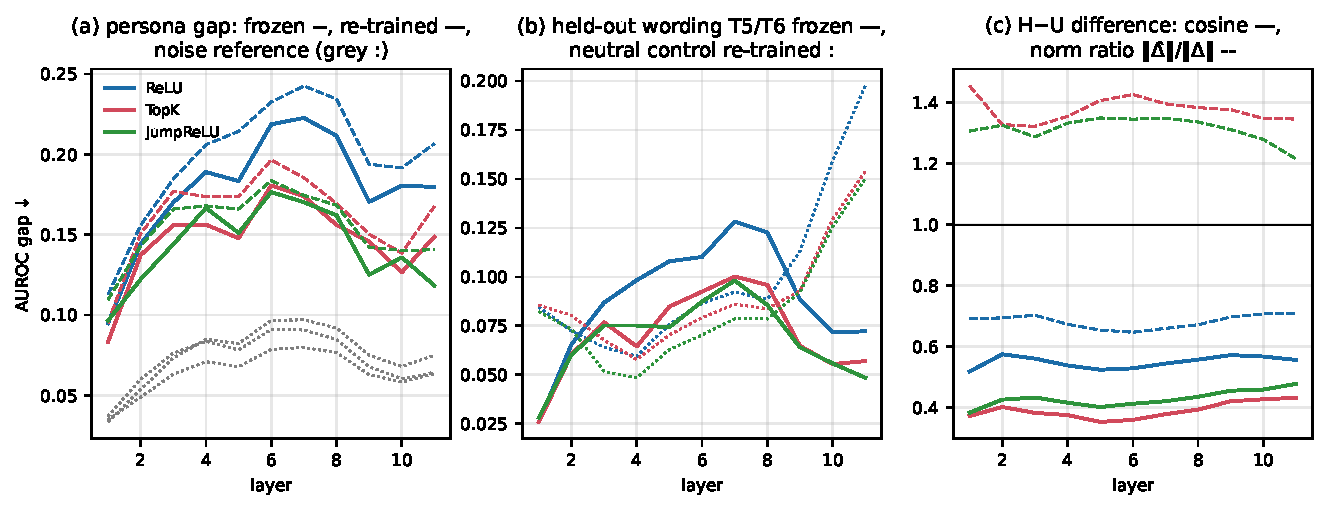
\includegraphics[width=\linewidth]{fig_rlm_layers}
  \caption{RLM-RP (\evlabel{validation}; 99 base SAEs, mean over 3 seeds). (a) Persona gaps: frozen logistic,
  re-trained logistic and the norm-matched noise reference. (b) Frozen gap on held-out wording T5/T6, and the re-trained
  gap on the neutral control. (c) Per-pair cosine and norm ratio between the reconstructed and original
  honest-minus-dishonest difference.}
  \label{fig:rlm}
\end{figure}

\clearpage
% generated by scripts/shared/build_paper_artifacts.py from results/geometry_of_truth/method_a_layer6/summary.csv, results/geometry_of_truth/e2e_inspired_layer6/summary.csv
\begin{table}[t]
\centering
\small
\caption{Layer-6 fine-tuning (VALIDATION; mean over 3 seeds). Method A lowered the B-MLP gap on 18/18 paired comparisons but never by more than 2 sd (pre-registered criterion not met). Output-KL rows for ReLU and JumpReLU fail the $\pm$5\% L0 guard and are not creditable. Source: \texttt{results/geometry\_of\_truth/method\_a\_layer6/summary.csv}; \texttt{results/geometry\_of\_truth/e2e\_inspired\_layer6/summary.csv}.}
\label{tab:ft6}
\begin{adjustbox}{max width=\linewidth}
\begin{tabular}{llccccc}
\toprule
SAE & Variant & GoT B-MLP gap $\downarrow$ & GoT rel. error $\downarrow$ & OWT EV $\uparrow$ & OWT $\Delta$CE $\downarrow$ & OWT L0 \\
\midrule
ReLU & Base & 0.321$\pm$0.022 & 0.059 & 0.828 & 0.177 & 134 \\
 & OWT-only control & 0.319$\pm$0.022 & 0.058 & 0.829 & 0.175 & 134 \\
 & Method A & 0.245$\pm$0.053 & 0.017 & 0.828 & 0.175 & 134 \\
 & Output-KL (B) & 0.280$\pm$0.020 & 0.024 & 0.830 & 0.145 & 141 \\
\midrule
TopK & Base & 0.203$\pm$0.030 & 0.034 & 0.853 & 0.104 & 128 \\
 & OWT-only control & 0.206$\pm$0.035 & 0.033 & 0.855 & 0.102 & 128 \\
 & Method A & 0.107$\pm$0.020 & 0.006 & 0.854 & 0.102 & 128 \\
 & Output-KL (B) & 0.114$\pm$0.022 & 0.009 & 0.852 & 0.091 & 128 \\
\midrule
JumpReLU & Base & 0.292$\pm$0.026 & 0.052 & 0.862 & 0.092 & 131 \\
 & OWT-only control & 0.287$\pm$0.027 & 0.052 & 0.864 & 0.091 & 131 \\
 & Method A & 0.238$\pm$0.056 & 0.015 & 0.863 & 0.091 & 131 \\
 & Output-KL (B) & 0.281$\pm$0.046 & 0.022 & 0.865 & 0.076 & 140 \\
\bottomrule
\end{tabular}
\end{adjustbox}
\end{table}

% generated by scripts/shared/build_paper_artifacts.py from results/geometry_of_truth/multilayer_finetune/criteria.json
\begin{table}[t]
\centering
\small
\caption{IMP-L pre-registered classifications (VALIDATION; 3 seeds). ``Consistent'' requires improvement on all 3 seeds and a mean paired difference larger than 2 sd; NOT CREDITABLE means a guard failed. $^\dagger$ original truth probe below the 0.70 informative threshold, so truth results are descriptive. Source: \texttt{results/\allowbreak{}geometry\_of\_truth/\allowbreak{}multilayer\_finetune/\allowbreak{}criteria.json}.}
\label{tab:impl_summary}
\begin{adjustbox}{max width=\linewidth}
\begin{tabular}{llccccc}
\toprule
Layer & SAE & Method A: truth & failed guards & Output-KL: behaviour & Output-KL: truth & failed guards \\
\midrule
3 & ReLU & NO IMPROVEMENT & -- & PRELIMINARY IMPROVEMENT & REGRESSION & -- \\
 & TopK & PRELIMINARY IMPROVEMENT & -- & PRELIMINARY IMPROVEMENT & REGRESSION & -- \\
 & JumpReLU & NO IMPROVEMENT & -- & PRELIMINARY IMPROVEMENT & NO IMPROVEMENT & -- \\
\midrule
8 & ReLU & PRELIMINARY IMPROVEMENT & -- & NOT CREDITABLE (guard failed) & NOT CREDITABLE (guard failed) & L0 $\pm$5\% \\
 & TopK & NO IMPROVEMENT & -- & PRELIMINARY IMPROVEMENT & NO IMPROVEMENT & -- \\
 & JumpReLU & NO IMPROVEMENT & -- & NOT CREDITABLE (guard failed) & NOT CREDITABLE (guard failed) & L0 $\pm$5\% \\
\midrule
9 & ReLU & PRELIMINARY IMPROVEMENT & -- & NOT CREDITABLE (guard failed) & NOT CREDITABLE (guard failed) & L0 $\pm$5\% \\
 & TopK & NO IMPROVEMENT & -- & PRELIMINARY IMPROVEMENT & NO IMPROVEMENT & -- \\
 & JumpReLU & PRELIMINARY IMPROVEMENT & -- & NOT CREDITABLE (guard failed) & NOT CREDITABLE (guard failed) & L0 $\pm$5\% \\
\bottomrule
\end{tabular}
\end{adjustbox}
\end{table}

% generated by scripts/shared/build_paper_artifacts.py from results/geometry_of_truth/multilayer_finetune/comparisons.csv, results/geometry_of_truth/multilayer_finetune/summary.csv, results/geometry_of_truth/multilayer_finetune/criteria.json
\begin{table}[t]
\centering
\small
\caption{IMP-L sparsity by dataset (VALIDATION; mean over 3 seeds): base L0 and the percentage change of each fine-tune, in the order OWT / GoT geographic / GoT numerical / RepE-LM persona prompts. Bold: $|\Delta| > 5\%$. The pre-registered guard is on OWT only; $^\ast$: output-KL failed it (excluded from rankings). TopK is fixed at 128 on every dataset. Source: \texttt{results/\allowbreak{}geometry\_of\_truth/\allowbreak{}multilayer\_finetune/\allowbreak{}comparisons.csv}; \texttt{results/\allowbreak{}geometry\_of\_truth/\allowbreak{}multilayer\_finetune/\allowbreak{}summary.csv}; \texttt{results/\allowbreak{}geometry\_of\_truth/\allowbreak{}multilayer\_finetune/\allowbreak{}criteria.json}.}
\label{tab:impl_l0}
\begin{adjustbox}{max width=\linewidth}
\begin{tabular}{llcccc}
\toprule
Layer & SAE & Base L0 (OWT / GoT geo. / GoT num. / RepE-LM) & OWT-only $\Delta$\% & Method A $\Delta$\% & Output-KL $\Delta$\% \\
\midrule
3 & ReLU & 134 / 45 / 56 / 189 & -0.2 / -2.2 / +0.0 / -0.3 & -0.2 / \textbf{-15.3} / \textbf{-27.5} / -0.2 & +3.5 / \textbf{-16.8} / \textbf{-25.3} / +4.6 \\
 & TopK & 128 / 128 / 128 / 128 & +0.0 / +0.0 / +0.0 / +0.0 & +0.0 / +0.0 / +0.0 / +0.0 & +0.0 / +0.0 / +0.0 / +0.0 \\
 & JumpReLU & 131 / 29 / 32 / 200 & +0.0 / -0.1 / -0.6 / +0.1 & +0.1 / \textbf{-9.0} / \textbf{-13.7} / +0.1 & +4.6 / \textbf{-5.5} / \textbf{-9.3} / +4.3 \\
\midrule
8 & ReLU & 134 / 77 / 97 / 161 & +0.1 / +1.7 / +0.9 / +0.0 & +0.1 / \textbf{-13.0} / \textbf{-17.1} / -0.1 & \textbf{+5.8} / \textbf{-22.6} / \textbf{-27.8} / \textbf{+6.2}$^\ast$ \\
 & TopK & 128 / 128 / 128 / 128 & +0.0 / +0.0 / +0.0 / +0.0 & +0.0 / +0.0 / +0.0 / +0.0 & +0.0 / +0.0 / +0.0 / +0.0 \\
 & JumpReLU & 132 / 63 / 63 / 167 & +0.4 / +0.5 / +0.4 / +0.4 & +0.3 / \textbf{-9.1} / \textbf{-7.5} / +0.5 & \textbf{+8.1} / \textbf{-14.3} / \textbf{-16.1} / \textbf{+8.1}$^\ast$ \\
\midrule
9 & ReLU & 135 / 110 / 90 / 162 & +0.2 / +0.6 / +1.4 / +0.1 & +0.1 / \textbf{-20.5} / \textbf{-11.7} / +0.1 & \textbf{+5.3} / \textbf{-29.5} / \textbf{-25.4} / \textbf{+5.8}$^\ast$ \\
 & TopK & 128 / 128 / 128 / 128 & +0.0 / +0.0 / +0.0 / +0.0 & +0.0 / +0.0 / +0.0 / +0.0 & +0.0 / +0.0 / +0.0 / +0.0 \\
 & JumpReLU & 132 / 71 / 66 / 160 & +0.4 / +0.7 / +1.0 / +0.5 & +0.3 / \textbf{-13.2} / \textbf{-8.8} / +0.6 & \textbf{+8.1} / \textbf{-17.9} / \textbf{-12.6} / \textbf{+8.6}$^\ast$ \\
\bottomrule
\end{tabular}
\end{adjustbox}
\end{table}


\begin{figure}[ht]
  \centering
  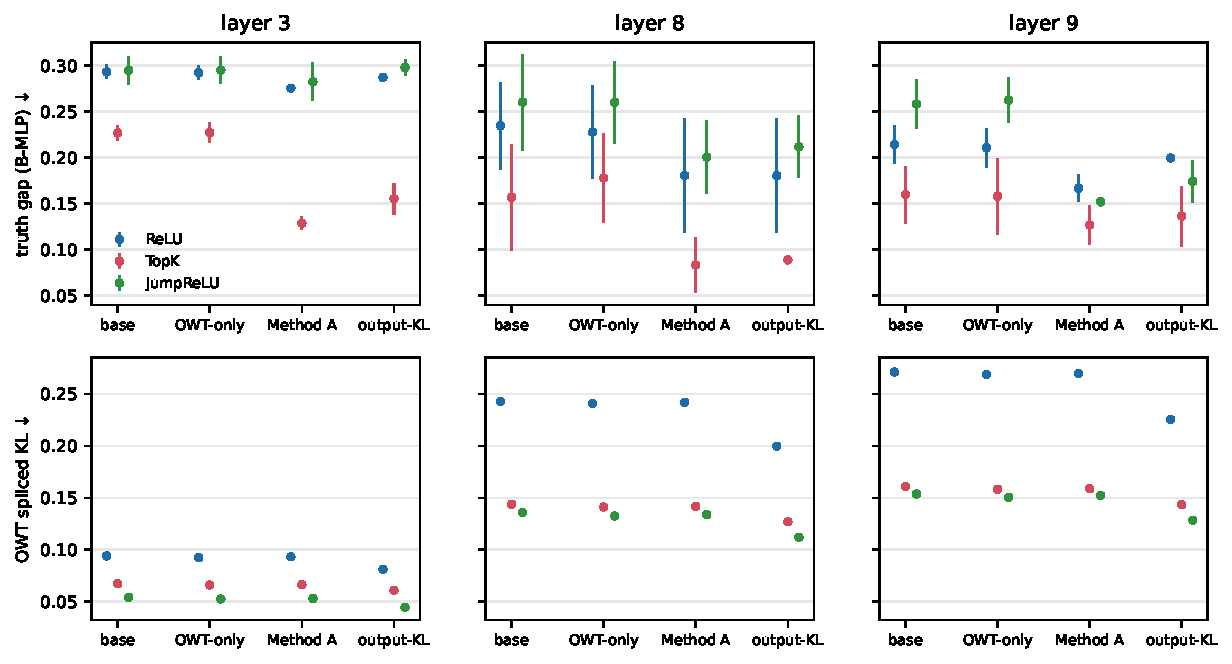
\includegraphics[width=\linewidth]{fig_impl_multilayer.pdf}
  \caption{IMP-L per-arm means ($\pm$1 sd over 3 seeds) of the independent truth gap (top) and OWT spliced KL (bottom)
  at layers 3, 8 and 9 (\evlabel{validation}). Output-KL points for ReLU and JumpReLU at layers 8 and 9 violate the
  pre-registered L0 guard. Source: \texttt{results/\allowbreak{}geometry\_of\_truth/\allowbreak{}multilayer\_finetune/\allowbreak{}summary.csv}.}
  \label{fig:impl}
\end{figure}

% generated by scripts/shared/build_paper_artifacts.py from results/geometry_of_truth/multilayer_finetune/comparisons.csv, results/geometry_of_truth/multilayer_finetune/summary.csv
\begin{table}[t]
\centering
\small
\caption{IMP-L at layer 3 (VALIDATION): paired differences over 3 seeds, mean [95\% $t$-interval]; relative error and L0 as mean percentage change. Lower is better except OWT EV. Source: \texttt{results/geometry\_of\_truth/multilayer\_finetune/comparisons.csv}; \texttt{results/geometry\_of\_truth/multilayer\_finetune/summary.csv}.}
\label{tab:impl3}
\begin{adjustbox}{max width=\linewidth}
\begin{tabular}{lccccccc}
\toprule
Comparison & Truth gap (B-MLP) & GoT rel.\ error & OWT EV & OWT $\Delta$CE & OWT KL & GoT stmt.\ KL & OWT L0 \\
\midrule
\multicolumn{8}{l}{\textbf{ReLU}: base truth gap 0.293, OWT EV 0.904, $\Delta$CE 0.078, OWT L0 134.0} \\
\quad owt\_only - base & \shortstack{-0.001\\ \scriptsize[-0.006, +0.004]} & -1.5\% & \shortstack{+0.001\\ \scriptsize[+0.001, +0.002]} & \shortstack{-0.002\\ \scriptsize[-0.005, +0.002]} & \shortstack{-0.002\\ \scriptsize[-0.003, -0.000]} & \shortstack{-0.002\\ \scriptsize[-0.006, +0.002]} & -0.2\% \\
\quad method\_a - base & \shortstack{-0.018\\ \scriptsize[-0.041, +0.005]} & -62.0\% & \shortstack{+0.001\\ \scriptsize[+0.000, +0.001]} & \shortstack{-0.001\\ \scriptsize[-0.005, +0.003]} & \shortstack{-0.001\\ \scriptsize[-0.002, +0.000]} & \shortstack{-0.001\\ \scriptsize[-0.007, +0.004]} & -0.2\% \\
\quad method\_a - owt\_only & \shortstack{-0.017\\ \scriptsize[-0.040, +0.007]} & -61.4\% & \shortstack{-0.001\\ \scriptsize[-0.001, -0.001]} & \shortstack{+0.001\\ \scriptsize[-0.000, +0.002]} & \shortstack{+0.001\\ \scriptsize[+0.000, +0.001]} & \shortstack{+0.000\\ \scriptsize[-0.003, +0.004]} & +0.0\% \\
\quad kl - base & \shortstack{-0.006\\ \scriptsize[-0.021, +0.009]} & -50.0\% & \shortstack{+0.001\\ \scriptsize[+0.001, +0.001]} & \shortstack{-0.009\\ \scriptsize[-0.013, -0.005]} & \shortstack{-0.013\\ \scriptsize[-0.015, -0.011]} & \shortstack{-0.052\\ \scriptsize[-0.058, -0.046]} & +3.5\% \\
\quad kl - method\_a & \shortstack{+0.012\\ \scriptsize[-0.000, +0.024]} & +31.5\% & \shortstack{+0.000\\ \scriptsize[+0.000, +0.001]} & \shortstack{-0.008\\ \scriptsize[-0.012, -0.004]} & \shortstack{-0.012\\ \scriptsize[-0.014, -0.010]} & \shortstack{-0.050\\ \scriptsize[-0.051, -0.049]} & +3.7\% \\
\midrule
\multicolumn{8}{l}{\textbf{TopK}: base truth gap 0.227, OWT EV 0.904, $\Delta$CE 0.057, OWT L0 128.0} \\
\quad owt\_only - base & \shortstack{+0.000\\ \scriptsize[-0.008, +0.009]} & -3.8\% & \shortstack{+0.002\\ \scriptsize[+0.002, +0.002]} & \shortstack{-0.001\\ \scriptsize[-0.003, +0.001]} & \shortstack{-0.001\\ \scriptsize[-0.002, -0.000]} & \shortstack{-0.000\\ \scriptsize[-0.001, +0.001]} & +0.0\% \\
\quad method\_a - base & \shortstack{-0.098\\ \scriptsize[-0.107, -0.089]} & -74.0\% & \shortstack{+0.001\\ \scriptsize[+0.001, +0.001]} & \shortstack{-0.001\\ \scriptsize[-0.002, +0.000]} & \shortstack{-0.001\\ \scriptsize[-0.002, -0.000]} & \shortstack{-0.000\\ \scriptsize[-0.001, +0.001]} & +0.0\% \\
\quad method\_a - owt\_only & \shortstack{-0.098\\ \scriptsize[-0.116, -0.081]} & -73.0\% & \shortstack{-0.000\\ \scriptsize[-0.001, -0.000]} & \shortstack{+0.000\\ \scriptsize[-0.001, +0.001]} & \shortstack{+0.000\\ \scriptsize[-0.000, +0.001]} & \shortstack{+0.000\\ \scriptsize[-0.002, +0.002]} & +0.0\% \\
\quad kl - base & \shortstack{-0.072\\ \scriptsize[-0.104, -0.039]} & -62.0\% & \shortstack{-0.001\\ \scriptsize[-0.001, -0.000]} & \shortstack{-0.003\\ \scriptsize[-0.005, -0.002]} & \shortstack{-0.006\\ \scriptsize[-0.007, -0.005]} & \shortstack{-0.036\\ \scriptsize[-0.043, -0.030]} & +0.0\% \\
\quad kl - method\_a & \shortstack{+0.027\\ \scriptsize[-0.001, +0.054]} & +46.2\% & \shortstack{-0.002\\ \scriptsize[-0.002, -0.002]} & \shortstack{-0.002\\ \scriptsize[-0.003, -0.002]} & \shortstack{-0.005\\ \scriptsize[-0.006, -0.005]} & \shortstack{-0.036\\ \scriptsize[-0.043, -0.030]} & +0.0\% \\
\midrule
\multicolumn{8}{l}{\textbf{JumpReLU}: base truth gap 0.294, OWT EV 0.914, $\Delta$CE 0.040, OWT L0 131.2} \\
\quad owt\_only - base & \shortstack{+0.000\\ \scriptsize[-0.014, +0.015]} & -1.4\% & \shortstack{+0.002\\ \scriptsize[+0.001, +0.002]} & \shortstack{-0.001\\ \scriptsize[-0.005, +0.002]} & \shortstack{-0.002\\ \scriptsize[-0.003, -0.001]} & \shortstack{-0.001\\ \scriptsize[-0.005, +0.002]} & +0.0\% \\
\quad method\_a - base & \shortstack{-0.012\\ \scriptsize[-0.043, +0.019]} & -61.1\% & \shortstack{+0.001\\ \scriptsize[+0.001, +0.001]} & \shortstack{-0.000\\ \scriptsize[-0.003, +0.002]} & \shortstack{-0.001\\ \scriptsize[-0.001, -0.001]} & \shortstack{-0.001\\ \scriptsize[-0.002, +0.000]} & +0.1\% \\
\quad method\_a - owt\_only & \shortstack{-0.013\\ \scriptsize[-0.031, +0.005]} & -60.5\% & \shortstack{-0.001\\ \scriptsize[-0.001, -0.001]} & \shortstack{+0.001\\ \scriptsize[-0.000, +0.002]} & \shortstack{+0.001\\ \scriptsize[-0.001, +0.002]} & \shortstack{+0.000\\ \scriptsize[-0.002, +0.002]} & +0.1\% \\
\quad kl - base & \shortstack{+0.003\\ \scriptsize[-0.013, +0.019]} & -48.8\% & \shortstack{+0.002\\ \scriptsize[+0.002, +0.002]} & \shortstack{-0.006\\ \scriptsize[-0.010, -0.002]} & \shortstack{-0.010\\ \scriptsize[-0.011, -0.008]} & \shortstack{-0.038\\ \scriptsize[-0.050, -0.026]} & +4.6\% \\
\quad kl - method\_a & \shortstack{+0.016\\ \scriptsize[-0.017, +0.048]} & +31.5\% & \shortstack{+0.001\\ \scriptsize[+0.001, +0.001]} & \shortstack{-0.005\\ \scriptsize[-0.007, -0.003]} & \shortstack{-0.009\\ \scriptsize[-0.010, -0.007]} & \shortstack{-0.037\\ \scriptsize[-0.048, -0.026]} & +4.5\% \\
\bottomrule
\end{tabular}
\end{adjustbox}
\end{table}

% generated by scripts/shared/build_paper_artifacts.py from results/geometry_of_truth/multilayer_finetune/comparisons.csv, results/geometry_of_truth/multilayer_finetune/summary.csv
\begin{table}[t]
\centering
\small
\caption{IMP-L at layer 8 (VALIDATION): paired differences over 3 seeds, mean [95\% $t$-interval]; relative error and L0 as mean percentage change. Lower is better except OWT EV. Source: \texttt{results/\allowbreak{}geometry\_of\_truth/\allowbreak{}multilayer\_finetune/\allowbreak{}comparisons.csv}; \texttt{results/\allowbreak{}geometry\_of\_truth/\allowbreak{}multilayer\_finetune/\allowbreak{}summary.csv}.}
\label{tab:impl8}
\begin{adjustbox}{max width=\linewidth}
\begin{tabular}{lccccccc}
\toprule
Comparison & Truth gap (B-MLP) & GoT rel.\ error & OWT EV & OWT $\Delta$CE & OWT KL & GoT stmt.\ KL & OWT L0 \\
\midrule
\multicolumn{8}{l}{\textbf{ReLU}: base truth gap 0.234, OWT EV 0.800, $\Delta$CE 0.223, OWT L0 134.5} \\
\quad owt\_only - base & \shortstack{-0.007\\ \scriptsize[-0.016, +0.002]} & -2.2\% & \shortstack{+0.001\\ \scriptsize[+0.001, +0.002]} & \shortstack{-0.002\\ \scriptsize[-0.002, -0.001]} & \shortstack{-0.002\\ \scriptsize[-0.003, -0.002]} & \shortstack{-0.001\\ \scriptsize[-0.003, +0.000]} & +0.1\% \\
\quad method\_a - base & \shortstack{-0.054\\ \scriptsize[-0.095, -0.013]} & -73.5\% & \shortstack{+0.001\\ \scriptsize[-0.000, +0.001]} & \shortstack{-0.001\\ \scriptsize[-0.002, -0.000]} & \shortstack{-0.001\\ \scriptsize[-0.002, -0.000]} & \shortstack{-0.003\\ \scriptsize[-0.006, +0.000]} & +0.1\% \\
\quad method\_a - owt\_only & \shortstack{-0.047\\ \scriptsize[-0.086, -0.008]} & -72.9\% & \shortstack{-0.001\\ \scriptsize[-0.001, -0.000]} & \shortstack{+0.001\\ \scriptsize[+0.001, +0.002]} & \shortstack{+0.001\\ \scriptsize[+0.001, +0.002]} & \shortstack{-0.002\\ \scriptsize[-0.004, +0.001]} & -0.0\% \\
\quad kl - base & \shortstack{-0.054\\ \scriptsize[-0.092, -0.016]} & -61.9\% & \shortstack{+0.003\\ \scriptsize[+0.002, +0.003]} & \shortstack{-0.039\\ \scriptsize[-0.041, -0.036]} & \shortstack{-0.043\\ \scriptsize[-0.045, -0.042]} & \shortstack{-0.154\\ \scriptsize[-0.238, -0.071]} & +5.8\% \\
\quad kl - method\_a & \shortstack{-0.000\\ \scriptsize[-0.037, +0.037]} & +43.9\% & \shortstack{+0.002\\ \scriptsize[+0.001, +0.003]} & \shortstack{-0.038\\ \scriptsize[-0.040, -0.036]} & \shortstack{-0.042\\ \scriptsize[-0.044, -0.041]} & \shortstack{-0.151\\ \scriptsize[-0.234, -0.069]} & +5.7\% \\
\midrule
\multicolumn{8}{l}{\textbf{TopK}: base truth gap 0.157, OWT EV 0.836, $\Delta$CE 0.126, OWT L0 128.0} \\
\quad owt\_only - base & \shortstack{+0.021\\ \scriptsize[-0.032, +0.074]} & -1.3\% & \shortstack{+0.002\\ \scriptsize[+0.002, +0.002]} & \shortstack{-0.002\\ \scriptsize[-0.004, -0.000]} & \shortstack{-0.003\\ \scriptsize[-0.004, -0.001]} & \shortstack{-0.002\\ \scriptsize[-0.008, +0.004]} & +0.0\% \\
\quad method\_a - base & \shortstack{-0.074\\ \scriptsize[-0.202, +0.054]} & -85.4\% & \shortstack{+0.001\\ \scriptsize[+0.001, +0.001]} & \shortstack{-0.003\\ \scriptsize[-0.004, -0.001]} & \shortstack{-0.002\\ \scriptsize[-0.004, -0.001]} & \shortstack{-0.001\\ \scriptsize[-0.004, +0.003]} & +0.0\% \\
\quad method\_a - owt\_only & \shortstack{-0.094\\ \scriptsize[-0.229, +0.040]} & -85.2\% & \shortstack{-0.001\\ \scriptsize[-0.001, -0.001]} & \shortstack{-0.001\\ \scriptsize[-0.002, +0.000]} & \shortstack{+0.000\\ \scriptsize[+0.000, +0.001]} & \shortstack{+0.002\\ \scriptsize[-0.005, +0.008]} & +0.0\% \\
\quad kl - base & \shortstack{-0.068\\ \scriptsize[-0.198, +0.062]} & -79.6\% & \shortstack{-0.002\\ \scriptsize[-0.002, -0.001]} & \shortstack{-0.017\\ \scriptsize[-0.021, -0.012]} & \shortstack{-0.017\\ \scriptsize[-0.018, -0.016]} & \shortstack{-0.079\\ \scriptsize[-0.103, -0.055]} & +0.0\% \\
\quad kl - method\_a & \shortstack{+0.006\\ \scriptsize[-0.065, +0.076]} & +40.2\% & \shortstack{-0.002\\ \scriptsize[-0.003, -0.002]} & \shortstack{-0.014\\ \scriptsize[-0.018, -0.010]} & \shortstack{-0.015\\ \scriptsize[-0.016, -0.014]} & \shortstack{-0.078\\ \scriptsize[-0.098, -0.058]} & +0.0\% \\
\midrule
\multicolumn{8}{l}{\textbf{JumpReLU}: base truth gap 0.260, OWT EV 0.840, $\Delta$CE 0.117, OWT L0 131.8} \\
\quad owt\_only - base & \shortstack{-0.000\\ \scriptsize[-0.025, +0.025]} & -0.7\% & \shortstack{+0.002\\ \scriptsize[+0.002, +0.003]} & \shortstack{-0.003\\ \scriptsize[-0.005, -0.001]} & \shortstack{-0.003\\ \scriptsize[-0.006, -0.001]} & \shortstack{-0.004\\ \scriptsize[-0.009, +0.002]} & +0.4\% \\
\quad method\_a - base & \shortstack{-0.060\\ \scriptsize[-0.247, +0.127]} & -79.6\% & \shortstack{+0.001\\ \scriptsize[+0.000, +0.001]} & \shortstack{-0.002\\ \scriptsize[-0.007, +0.002]} & \shortstack{-0.002\\ \scriptsize[-0.004, +0.000]} & \shortstack{+0.001\\ \scriptsize[-0.005, +0.007]} & +0.3\% \\
\quad method\_a - owt\_only & \shortstack{-0.060\\ \scriptsize[-0.238, +0.119]} & -79.4\% & \shortstack{-0.002\\ \scriptsize[-0.002, -0.001]} & \shortstack{+0.001\\ \scriptsize[-0.002, +0.004]} & \shortstack{+0.001\\ \scriptsize[+0.001, +0.002]} & \shortstack{+0.005\\ \scriptsize[-0.005, +0.016]} & -0.1\% \\
\quad kl - base & \shortstack{-0.048\\ \scriptsize[-0.164, +0.067]} & -69.4\% & \shortstack{+0.005\\ \scriptsize[+0.004, +0.005]} & \shortstack{-0.024\\ \scriptsize[-0.028, -0.020]} & \shortstack{-0.024\\ \scriptsize[-0.027, -0.021]} & \shortstack{-0.102\\ \scriptsize[-0.114, -0.089]} & +8.1\% \\
\quad kl - method\_a & \shortstack{+0.011\\ \scriptsize[-0.065, +0.087]} & +49.7\% & \shortstack{+0.004\\ \scriptsize[+0.004, +0.004]} & \shortstack{-0.021\\ \scriptsize[-0.022, -0.021]} & \shortstack{-0.022\\ \scriptsize[-0.024, -0.020]} & \shortstack{-0.103\\ \scriptsize[-0.121, -0.085]} & +7.8\% \\
\bottomrule
\end{tabular}
\end{adjustbox}
\end{table}

% generated by scripts/shared/build_paper_artifacts.py from results/geometry_of_truth/multilayer_finetune/comparisons.csv, results/geometry_of_truth/multilayer_finetune/summary.csv
\begin{table}[t]
\centering
\small
\caption{IMP-L at layer 9 (VALIDATION): paired differences over 3 seeds, mean [95\% $t$-interval]; relative error and L0 as mean percentage change. Lower is better except OWT EV. Source: \texttt{results/geometry\_of\_truth/multilayer\_finetune/comparisons.csv}; \texttt{results/geometry\_of\_truth/multilayer\_finetune/summary.csv}.}
\label{tab:impl9}
\begin{adjustbox}{max width=\linewidth}
\begin{tabular}{lccccccc}
\toprule
Comparison & Truth gap (B-MLP) & GoT rel.\ error & OWT EV & OWT $\Delta$CE & OWT KL & GoT stmt.\ KL & OWT L0 \\
\midrule
\multicolumn{8}{l}{\textbf{ReLU}: base truth gap 0.214, OWT EV 0.784, $\Delta$CE 0.250, OWT L0 135.0} \\
\quad owt\_only - base & \shortstack{-0.004\\ \scriptsize[-0.004, -0.003]} & -0.7\% & \shortstack{+0.001\\ \scriptsize[-0.000, +0.003]} & \shortstack{-0.002\\ \scriptsize[-0.003, -0.002]} & \shortstack{-0.002\\ \scriptsize[-0.004, -0.001]} & \shortstack{+0.001\\ \scriptsize[-0.009, +0.012]} & +0.2\% \\
\quad method\_a - base & \shortstack{-0.047\\ \scriptsize[-0.065, -0.030]} & -72.6\% & \shortstack{+0.001\\ \scriptsize[-0.001, +0.002]} & \shortstack{-0.002\\ \scriptsize[-0.003, -0.001]} & \shortstack{-0.001\\ \scriptsize[-0.003, +0.000]} & \shortstack{-0.005\\ \scriptsize[-0.022, +0.011]} & +0.1\% \\
\quad method\_a - owt\_only & \shortstack{-0.044\\ \scriptsize[-0.062, -0.026]} & -72.4\% & \shortstack{-0.001\\ \scriptsize[-0.001, -0.001]} & \shortstack{+0.000\\ \scriptsize[-0.001, +0.001]} & \shortstack{+0.001\\ \scriptsize[+0.000, +0.001]} & \shortstack{-0.007\\ \scriptsize[-0.014, +0.001]} & -0.1\% \\
\quad kl - base & \shortstack{-0.015\\ \scriptsize[-0.069, +0.040]} & -59.2\% & \shortstack{+0.002\\ \scriptsize[+0.000, +0.004]} & \shortstack{-0.042\\ \scriptsize[-0.044, -0.041]} & \shortstack{-0.046\\ \scriptsize[-0.048, -0.044]} & \shortstack{-0.208\\ \scriptsize[-0.230, -0.185]} & +5.3\% \\
\quad kl - method\_a & \shortstack{+0.033\\ \scriptsize[-0.006, +0.071]} & +49.1\% & \shortstack{+0.002\\ \scriptsize[+0.001, +0.002]} & \shortstack{-0.041\\ \scriptsize[-0.042, -0.039]} & \shortstack{-0.044\\ \scriptsize[-0.045, -0.043]} & \shortstack{-0.202\\ \scriptsize[-0.241, -0.164]} & +5.2\% \\
\midrule
\multicolumn{8}{l}{\textbf{TopK}: base truth gap 0.160, OWT EV 0.826, $\Delta$CE 0.150, OWT L0 128.0} \\
\quad owt\_only - base & \shortstack{-0.002\\ \scriptsize[-0.053, +0.050]} & -1.6\% & \shortstack{+0.002\\ \scriptsize[+0.002, +0.002]} & \shortstack{-0.002\\ \scriptsize[-0.003, -0.000]} & \shortstack{-0.003\\ \scriptsize[-0.003, -0.002]} & \shortstack{-0.002\\ \scriptsize[-0.009, +0.004]} & +0.0\% \\
\quad method\_a - base & \shortstack{-0.033\\ \scriptsize[-0.061, -0.005]} & -85.4\% & \shortstack{+0.001\\ \scriptsize[+0.001, +0.001]} & \shortstack{-0.002\\ \scriptsize[-0.003, -0.001]} & \shortstack{-0.002\\ \scriptsize[-0.003, -0.001]} & \shortstack{-0.003\\ \scriptsize[-0.008, +0.002]} & +0.0\% \\
\quad method\_a - owt\_only & \shortstack{-0.031\\ \scriptsize[-0.103, +0.041]} & -85.2\% & \shortstack{-0.001\\ \scriptsize[-0.001, -0.001]} & \shortstack{-0.000\\ \scriptsize[-0.001, -0.000]} & \shortstack{+0.000\\ \scriptsize[-0.000, +0.001]} & \shortstack{-0.000\\ \scriptsize[-0.002, +0.001]} & +0.0\% \\
\quad kl - base & \shortstack{-0.023\\ \scriptsize[-0.028, -0.018]} & -80.2\% & \shortstack{-0.002\\ \scriptsize[-0.002, -0.001]} & \shortstack{-0.015\\ \scriptsize[-0.017, -0.013]} & \shortstack{-0.018\\ \scriptsize[-0.018, -0.017]} & \shortstack{-0.084\\ \scriptsize[-0.119, -0.049]} & +0.0\% \\
\quad kl - method\_a & \shortstack{+0.010\\ \scriptsize[-0.024, +0.043]} & +35.3\% & \shortstack{-0.002\\ \scriptsize[-0.002, -0.002]} & \shortstack{-0.013\\ \scriptsize[-0.016, -0.010]} & \shortstack{-0.015\\ \scriptsize[-0.016, -0.014]} & \shortstack{-0.081\\ \scriptsize[-0.112, -0.050]} & +0.0\% \\
\midrule
\multicolumn{8}{l}{\textbf{JumpReLU}: base truth gap 0.258, OWT EV 0.829, $\Delta$CE 0.140, OWT L0 131.9} \\
\quad owt\_only - base & \shortstack{+0.004\\ \scriptsize[-0.038, +0.047]} & -1.1\% & \shortstack{+0.002\\ \scriptsize[+0.002, +0.003]} & \shortstack{-0.004\\ \scriptsize[-0.008, +0.001]} & \shortstack{-0.003\\ \scriptsize[-0.005, -0.002]} & \shortstack{-0.003\\ \scriptsize[-0.011, +0.004]} & +0.4\% \\
\quad method\_a - base & \shortstack{-0.106\\ \scriptsize[-0.162, -0.050]} & -78.7\% & \shortstack{+0.001\\ \scriptsize[-0.000, +0.001]} & \shortstack{-0.002\\ \scriptsize[-0.008, +0.004]} & \shortstack{-0.002\\ \scriptsize[-0.003, -0.000]} & \shortstack{-0.003\\ \scriptsize[-0.007, +0.001]} & +0.3\% \\
\quad method\_a - owt\_only & \shortstack{-0.110\\ \scriptsize[-0.169, -0.051]} & -78.5\% & \shortstack{-0.002\\ \scriptsize[-0.002, -0.002]} & \shortstack{+0.002\\ \scriptsize[-0.000, +0.004]} & \shortstack{+0.002\\ \scriptsize[+0.001, +0.002]} & \shortstack{+0.000\\ \scriptsize[-0.006, +0.006]} & -0.1\% \\
\quad kl - base & \shortstack{-0.084\\ \scriptsize[-0.095, -0.073]} & -70.4\% & \shortstack{+0.005\\ \scriptsize[+0.004, +0.005]} & \shortstack{-0.023\\ \scriptsize[-0.028, -0.017]} & \shortstack{-0.025\\ \scriptsize[-0.027, -0.024]} & \shortstack{-0.115\\ \scriptsize[-0.149, -0.080]} & +8.1\% \\
\quad kl - method\_a & \shortstack{+0.022\\ \scriptsize[-0.024, +0.068]} & +39.3\% & \shortstack{+0.004\\ \scriptsize[+0.004, +0.005]} & \shortstack{-0.021\\ \scriptsize[-0.022, -0.020]} & \shortstack{-0.024\\ \scriptsize[-0.026, -0.022]} & \shortstack{-0.112\\ \scriptsize[-0.148, -0.075]} & +7.7\% \\
\bottomrule
\end{tabular}
\end{adjustbox}
\end{table}

\clearpage
% generated by scripts/shared/build_paper_artifacts.py from results/repe/e3_finetuned_causal_preservation/hypotheses.csv, results/repe/e3_finetuned_causal_preservation/site_reconstruction.csv
\begin{table}[t]
\centering
\small
\caption{E3: causal preservation at the layer-8 final token for the base and IMP-L fine-tuned SAEs (VALIDATION; RepE-LM T2--T4; $T_{\text{full}}=0.0220$ nats, identical for all 36 SAEs; mean$\pm$sd over 3 seeds). $T_{\text{rec}}-S_{\text{rec}}$: persona minus synonym restoration (specificity). H4a/H4c: seeds passing the M4 control tests (reconstruction above matched-norm and decoder-shuffle vectors; top-$k^\ast$ features above 200 matched random sets). Site EV and L0 on RepE-LM validation prompts. Source: \texttt{results/\allowbreak{}repe/\allowbreak{}e3\_finetuned\_causal\_preservation/\allowbreak{}hypotheses.csv}; \texttt{results/\allowbreak{}repe/\allowbreak{}e3\_finetuned\_causal\_preservation/\allowbreak{}site\_reconstruction.csv}.}
\label{tab:e3}
\begin{adjustbox}{max width=\linewidth}
\begin{tabular}{llccccccccc}
\toprule
SAE & Arm & $T_{\text{rec}}/T_{\text{full}}$ & per seed (42, 1042, 2042) & $T_{\text{rec}}$ (nats) & $T_{\text{err}}/T_{\text{full}}$ & $|I|/T_{\text{full}}$ & $T_{\text{rec}}-S_{\text{rec}}$ & H4a/H4c seeds & site EV & site L0 \\
\midrule
ReLU & base & 0.621$\pm$0.015 & (0.630, 0.604, 0.630) & 0.0137$\pm$0.0003 & 0.450 & 0.117 & +0.0062 & 3/3 & 0.752 & 161 \\
 & OWT-only & 0.621$\pm$0.016 & (0.627, 0.603, 0.633) & 0.0137$\pm$0.0004 & 0.450 & 0.117 & +0.0062 & 3/3 & 0.753 & 161 \\
 & Method A & 0.622$\pm$0.016 & (0.623, 0.605, 0.636) & 0.0137$\pm$0.0003 & 0.449 & 0.117 & +0.0063 & 3/3 & 0.752 & 161 \\
 & output-KL & 0.640$\pm$0.016 & (0.645, 0.621, 0.653) & 0.0141$\pm$0.0004 & 0.426 & 0.114 & +0.0065 & 3/3 & 0.757 & 171 \\
\midrule
TopK & base & 0.625$\pm$0.039 & (0.580, 0.650, 0.645) & 0.0138$\pm$0.0009 & 0.094 & 0.323 & +0.0070 & 3/3 & 0.781 & 128 \\
 & OWT-only & 0.632$\pm$0.024 & (0.604, 0.650, 0.640) & 0.0139$\pm$0.0005 & 0.083 & 0.326 & +0.0073 & 3/3 & 0.784 & 128 \\
 & Method A & 0.615$\pm$0.005 & (0.611, 0.613, 0.620) & 0.0135$\pm$0.0001 & 0.091 & 0.330 & +0.0068 & 3/3 & 0.782 & 128 \\
 & output-KL & 0.619$\pm$0.037 & (0.577, 0.638, 0.643) & 0.0136$\pm$0.0008 & 0.074 & 0.336 & +0.0072 & 3/3 & 0.779 & 128 \\
\midrule
JumpReLU & base & 0.665$\pm$0.011 & (0.653, 0.665, 0.676) & 0.0146$\pm$0.0002 & 0.111 & 0.264 & +0.0074 & 3/3 & 0.811 & 167 \\
 & OWT-only & 0.669$\pm$0.029 & (0.648, 0.658, 0.702) & 0.0147$\pm$0.0006 & 0.111 & 0.255 & +0.0074 & 3/3 & 0.815 & 168 \\
 & Method A & 0.668$\pm$0.025 & (0.639, 0.685, 0.681) & 0.0147$\pm$0.0006 & 0.101 & 0.265 & +0.0075 & 3/3 & 0.813 & 168 \\
 & output-KL & 0.687$\pm$0.014 & (0.673, 0.687, 0.701) & 0.0151$\pm$0.0003 & 0.059 & 0.285 & +0.0080 & 3/3 & 0.819 & 181 \\
\bottomrule
\end{tabular}
\end{adjustbox}
\end{table}

% generated by scripts/shared/build_paper_artifacts.py from results/repe/e3_finetuned_causal_preservation/comparisons.csv, results/repe/e3_finetuned_causal_preservation/criteria.json
\begin{table}[t]
\centering
\small
\caption{E3 paired comparisons of $T_{\text{rec}}/T_{\text{full}}$ ($\uparrow$; VALIDATION; 3 seeds; 95\% $t$-interval, df 2) and the pre-registered classes: E3-H1 (Method A, consistent against both base and OWT-only; class shown on the second row) and E3-H2 (output-KL vs Method A; NOT CREDITABLE a priori for ReLU and JumpReLU, whose IMP-L L0 guard failed). Source: \texttt{results/\allowbreak{}repe/\allowbreak{}e3\_finetuned\_causal\_preservation/\allowbreak{}comparisons.csv}; \texttt{results/\allowbreak{}repe/\allowbreak{}e3\_finetuned\_causal\_preservation/\allowbreak{}criteria.json}.}
\label{tab:e3_classes}
\begin{adjustbox}{max width=\linewidth}
\begin{tabular}{llccccl}
\toprule
SAE & Comparison & $\Delta$ preservation & 95\% CI & per seed & $\Delta(T_{\text{rec}}-S_{\text{rec}})$ & pre-registered class \\
\midrule
ReLU & method\_a - base & +0.0002 & [-0.0166, +0.0170] & (-0.007, +0.001, +0.007) & +0.00001 &  \\
 & method\_a - owt\_only & +0.0006 & [-0.0092, +0.0104] & (-0.004, +0.002, +0.003) & +0.00003 & NO IMPROVEMENT \\
 & kl - method\_a & +0.0180 & [+0.0107, +0.0252] & (+0.021, +0.016, +0.016) & +0.00022 & NOT CREDITABLE (guard failed) \\
 & owt\_only - base & -0.0004 & [-0.0087, +0.0078] & (-0.003, -0.002, +0.003) & -0.00001 &  \\
 & kl - base & +0.0182 & [+0.0075, +0.0288] & (+0.015, +0.017, +0.023) & +0.00023 &  \\
\midrule
TopK & method\_a - base & -0.0101 & [-0.1005, +0.0803] & (+0.031, -0.037, -0.025) & -0.00017 &  \\
 & method\_a - owt\_only & -0.0169 & [-0.0714, +0.0375] & (+0.007, -0.037, -0.020) & -0.00045 & NO IMPROVEMENT \\
 & kl - method\_a & +0.0046 & [-0.0783, +0.0876] & (-0.034, +0.025, +0.023) & +0.00040 & NO IMPROVEMENT \\
 & owt\_only - base & +0.0068 & [-0.0323, +0.0460] & (+0.025, +0.000, -0.005) & +0.00029 &  \\
 & kl - base & -0.0055 & [-0.0196, +0.0086] & (-0.003, -0.012, -0.002) & +0.00024 &  \\
\midrule
JumpReLU & method\_a - base & +0.0040 & [-0.0388, +0.0468] & (-0.014, +0.020, +0.005) & +0.00012 &  \\
 & method\_a - owt\_only & -0.0008 & [-0.0615, +0.0598] & (-0.008, +0.026, -0.021) & +0.00011 & NO IMPROVEMENT \\
 & kl - method\_a & +0.0184 & [-0.0204, +0.0572] & (+0.033, +0.002, +0.019) & +0.00050 & NOT CREDITABLE (guard failed) \\
 & owt\_only - base & +0.0048 & [-0.0410, +0.0506] & (-0.006, -0.006, +0.026) & +0.00002 &  \\
 & kl - base & +0.0223 & [+0.0156, +0.0291] & (+0.019, +0.023, +0.025) & +0.00062 &  \\
\bottomrule
\end{tabular}
\end{adjustbox}
\end{table}


\begin{figure}[ht]
  \centering
  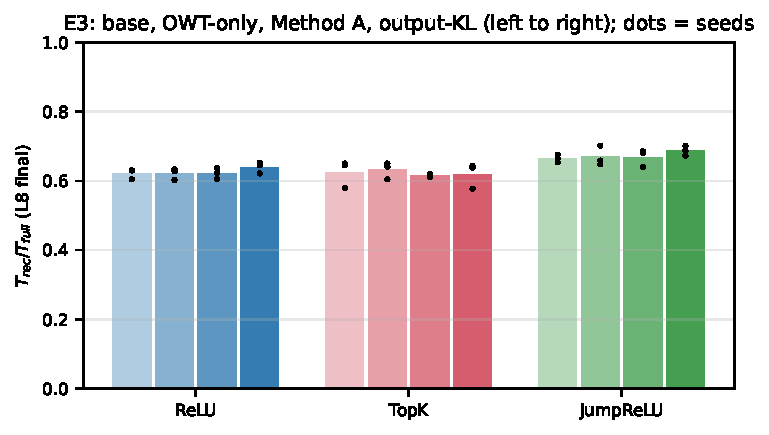
\includegraphics[width=0.7\linewidth]{fig_e3_preservation}
  \caption{E3 (\evlabel{validation}): share of the persona-instruction effect carried by the SAE reconstruction at the
  layer-8 final token for base, OWT-only, Method A and output-KL SAEs (bars: mean of 3 seeds; dots: seeds). Output-KL
  ReLU and JumpReLU violate the pre-registered L0 guard.}
  \label{fig:e3}
\end{figure}

\clearpage
% generated by scripts/shared/build_paper_artifacts.py from results/openwebtext/r2_scaled_saes/comparisons.csv
\begin{table}[t]
\centering
\small
\caption{R2 before/after, TopK-3072 (old) $\rightarrow$ TopK-12288 (R2) (VALIDATION; L0 = 128 $\pm$ 10\% on OWT; mean$\pm$sd). Improvement: positive = better. Class: IMPROVEMENT if all 9 new/old seed pairs favour R2 and the Welch interval excludes 0 (pre-registered). GoT is evaluated at layers 8 and 11 only. Source: \texttt{results/\allowbreak{}openwebtext/\allowbreak{}r2\_scaled\_saes/\allowbreak{}comparisons.csv}.}
\label{tab:r2_c1}
\begin{adjustbox}{max width=\linewidth}
\begin{tabular}{llccccl}
\toprule
Layer & Metric & Before (old, 3 seeds) & After (R2, 3 seeds) & $\Delta$ [Welch 95\% CI] & Improvement & Class \\
\midrule
L1 & OWT NMSE $\downarrow$ & 0.0811$\pm$0.0004 & 0.0255$\pm$0.0001 & -0.0556 [-0.0567, -0.0545] & +68.5\% & IMPROVEMENT \\
 & spliced $\Delta$CE $\downarrow$ & 0.0256$\pm$0.0015 & 0.0063$\pm$0.0008 & -0.0193 [-0.0224, -0.0161] & +75.3\% & IMPROVEMENT \\
 & spliced KL $\downarrow$ & 0.0288$\pm$0.0013 & 0.0073$\pm$0.0001 & -0.0215 [-0.0247, -0.0184] & +74.7\% & IMPROVEMENT \\
 & persona re-fit gap $\downarrow$ & 0.083$\pm$0.012 & 0.067$\pm$0.003 & -0.016 [-0.045, +0.012] & +19.8\% & no clear change \\
 & persona SAE$-$PCA gap $\downarrow$ & 0.007$\pm$0.012 & 0.021$\pm$0.003 & +0.014 [-0.015, +0.043] & -- & no clear change \\
 & pair-direction cos $\uparrow$ & 0.373$\pm$0.003 & 0.507$\pm$0.003 & +0.135 [+0.128, +0.141] & +36.1\% & IMPROVEMENT \\
 & $T_{\text{rec}}/T_{\text{full}}$ $\uparrow$ & 0.931$\pm$0.014 & 0.988$\pm$0.005 & +0.057 [+0.025, +0.088] & +6.1\% & IMPROVEMENT \\
\midrule
L8 & OWT NMSE $\downarrow$ & 0.1643$\pm$0.0005 & 0.0959$\pm$0.0001 & -0.0684 [-0.0696, -0.0671] & +41.6\% & IMPROVEMENT \\
 & spliced $\Delta$CE $\downarrow$ & 0.1259$\pm$0.0043 & 0.0603$\pm$0.0018 & -0.0656 [-0.0747, -0.0565] & +52.1\% & IMPROVEMENT \\
 & spliced KL $\downarrow$ & 0.1439$\pm$0.0019 & 0.0680$\pm$0.0002 & -0.0759 [-0.0806, -0.0712] & +52.8\% & IMPROVEMENT \\
 & persona re-fit gap $\downarrow$ & 0.156$\pm$0.017 & 0.108$\pm$0.009 & -0.048 [-0.082, -0.014] & +30.7\% & IMPROVEMENT \\
 & persona SAE$-$PCA gap $\downarrow$ & 0.033$\pm$0.017 & 0.027$\pm$0.009 & -0.006 [-0.041, +0.028] & -- & no clear change \\
 & GoT re-fit gap $\downarrow$ & 0.061$\pm$0.015 & 0.055$\pm$0.022 & -0.006 [-0.051, +0.040] & +9.0\% & no clear change \\
 & pair-direction cos $\uparrow$ & 0.394$\pm$0.003 & 0.488$\pm$0.001 & +0.094 [+0.086, +0.103] & +24.0\% & IMPROVEMENT \\
 & $T_{\text{rec}}/T_{\text{full}}$ $\uparrow$ & 0.625$\pm$0.039 & 0.726$\pm$0.020 & +0.101 [+0.019, +0.182] & +16.1\% & IMPROVEMENT \\
\midrule
L11 & OWT NMSE $\downarrow$ & 0.1891$\pm$0.0005 & 0.1129$\pm$0.0002 & -0.0762 [-0.0773, -0.0751] & +40.3\% & IMPROVEMENT \\
 & spliced $\Delta$CE $\downarrow$ & 0.2129$\pm$0.0018 & 0.0995$\pm$0.0011 & -0.1134 [-0.1171, -0.1097] & +53.3\% & IMPROVEMENT \\
 & spliced KL $\downarrow$ & 0.2177$\pm$0.0015 & 0.1034$\pm$0.0011 & -0.1143 [-0.1175, -0.1112] & +52.5\% & IMPROVEMENT \\
 & persona re-fit gap $\downarrow$ & 0.149$\pm$0.015 & 0.109$\pm$0.008 & -0.040 [-0.071, -0.008] & +26.7\% & IMPROVEMENT \\
 & persona SAE$-$PCA gap $\downarrow$ & 0.083$\pm$0.015 & 0.070$\pm$0.008 & -0.013 [-0.045, +0.019] & -- & no clear change \\
 & GoT re-fit gap $\downarrow$ & 0.110$\pm$0.015 & 0.100$\pm$0.030 & -0.010 [-0.073, +0.053] & +9.0\% & no clear change \\
 & pair-direction cos $\uparrow$ & 0.432$\pm$0.001 & 0.513$\pm$0.001 & +0.080 [+0.077, +0.083] & +18.6\% & IMPROVEMENT \\
 & $T_{\text{rec}}/T_{\text{full}}$ $\uparrow$ & 0.620$\pm$0.004 & 0.692$\pm$0.002 & +0.073 [+0.064, +0.082] & +11.8\% & IMPROVEMENT \\
\bottomrule
\end{tabular}
\end{adjustbox}
\end{table}

% generated by scripts/shared/build_paper_artifacts.py from results/openwebtext/r2_scaled_saes/comparisons.csv
\begin{table}[t]
\centering
\small
\caption{R2 before/after, ReLU-3072 (old) $\rightarrow$ ReLU-12288 (R2) (VALIDATION; L0 = 128 $\pm$ 10\% on OWT; mean$\pm$sd). Improvement: positive = better. Class: IMPROVEMENT if all 9 new/old seed pairs favour R2 and the Welch interval excludes 0 (pre-registered). GoT is evaluated at layers 8 and 11 only. Source: \texttt{results/\allowbreak{}openwebtext/\allowbreak{}r2\_scaled\_saes/\allowbreak{}comparisons.csv}.}
\label{tab:r2_c2}
\begin{adjustbox}{max width=\linewidth}
\begin{tabular}{llccccl}
\toprule
Layer & Metric & Before (old, 3 seeds) & After (R2, 3 seeds) & $\Delta$ [Welch 95\% CI] & Improvement & Class \\
\midrule
L1 & OWT NMSE $\downarrow$ & 0.0651$\pm$0.0005 & 0.0231$\pm$0.0001 & -0.0420 [-0.0431, -0.0410] & +64.5\% & IMPROVEMENT \\
 & spliced $\Delta$CE $\downarrow$ & 0.0191$\pm$0.0014 & 0.0035$\pm$0.0010 & -0.0156 [-0.0186, -0.0126] & +81.5\% & IMPROVEMENT \\
 & spliced KL $\downarrow$ & 0.0231$\pm$0.0005 & 0.0064$\pm$0.0001 & -0.0168 [-0.0179, -0.0156] & +72.4\% & IMPROVEMENT \\
 & persona re-fit gap $\downarrow$ & 0.095$\pm$0.006 & 0.089$\pm$0.005 & -0.006 [-0.018, +0.006] & +6.2\% & no clear change \\
 & persona SAE$-$PCA gap $\downarrow$ & 0.023$\pm$0.005 & 0.046$\pm$0.005 & +0.024 [+0.013, +0.034] & -- & \textbf{REGRESSION} \\
 & pair-direction cos $\uparrow$ & 0.519$\pm$0.006 & 0.602$\pm$0.005 & +0.084 [+0.071, +0.096] & +16.1\% & IMPROVEMENT \\
 & $T_{\text{rec}}/T_{\text{full}}$ $\uparrow$ & 0.938$\pm$0.019 & 0.992$\pm$0.005 & +0.054 [+0.010, +0.098] & +5.8\% & IMPROVEMENT \\
\midrule
L8 & OWT NMSE $\downarrow$ & 0.1997$\pm$0.0003 & 0.1334$\pm$0.0000 & -0.0662 [-0.0670, -0.0655] & +33.2\% & IMPROVEMENT \\
 & spliced $\Delta$CE $\downarrow$ & 0.2230$\pm$0.0034 & 0.1269$\pm$0.0007 & -0.0960 [-0.1039, -0.0881] & +43.1\% & IMPROVEMENT \\
 & spliced KL $\downarrow$ & 0.2431$\pm$0.0022 & 0.1424$\pm$0.0009 & -0.1007 [-0.1054, -0.0959] & +41.4\% & IMPROVEMENT \\
 & persona re-fit gap $\downarrow$ & 0.212$\pm$0.004 & 0.193$\pm$0.004 & -0.019 [-0.027, -0.010] & +8.9\% & IMPROVEMENT \\
 & persona SAE$-$PCA gap $\downarrow$ & 0.075$\pm$0.004 & 0.092$\pm$0.004 & +0.017 [+0.008, +0.025] & -- & \textbf{REGRESSION} \\
 & GoT re-fit gap $\downarrow$ & 0.034$\pm$0.011 & 0.012$\pm$0.005 & -0.022 [-0.044, +0.000] & +64.8\% & no clear change \\
 & pair-direction cos $\uparrow$ & 0.558$\pm$0.005 & 0.607$\pm$0.002 & +0.050 [+0.038, +0.061] & +8.9\% & IMPROVEMENT \\
 & $T_{\text{rec}}/T_{\text{full}}$ $\uparrow$ & 0.621$\pm$0.015 & 0.643$\pm$0.016 & +0.022 [-0.013, +0.056] & +3.5\% & no clear change \\
\midrule
L11 & OWT NMSE $\downarrow$ & 0.2484$\pm$0.0005 & 0.1706$\pm$0.0002 & -0.0778 [-0.0789, -0.0768] & +31.3\% & IMPROVEMENT \\
 & spliced $\Delta$CE $\downarrow$ & 0.3580$\pm$0.0024 & 0.2241$\pm$0.0030 & -0.1340 [-0.1402, -0.1277] & +37.4\% & IMPROVEMENT \\
 & spliced KL $\downarrow$ & 0.3685$\pm$0.0026 & 0.2307$\pm$0.0012 & -0.1378 [-0.1434, -0.1323] & +37.4\% & IMPROVEMENT \\
 & persona re-fit gap $\downarrow$ & 0.180$\pm$0.021 & 0.194$\pm$0.006 & +0.014 [-0.034, +0.062] & -7.8\% & no clear change \\
 & persona SAE$-$PCA gap $\downarrow$ & 0.104$\pm$0.021 & 0.137$\pm$0.006 & +0.033 [-0.015, +0.080] & -- & no clear change \\
 & GoT re-fit gap $\downarrow$ & 0.105$\pm$0.016 & 0.076$\pm$0.003 & -0.029 [-0.068, +0.009] & +27.8\% & no clear change \\
 & pair-direction cos $\uparrow$ & 0.557$\pm$0.003 & 0.622$\pm$0.002 & +0.066 [+0.059, +0.072] & +11.8\% & IMPROVEMENT \\
 & $T_{\text{rec}}/T_{\text{full}}$ $\uparrow$ & 0.677$\pm$0.014 & 0.712$\pm$0.005 & +0.036 [+0.005, +0.066] & +5.2\% & IMPROVEMENT \\
\bottomrule
\end{tabular}
\end{adjustbox}
\end{table}

% generated by scripts/shared/build_paper_artifacts.py from results/openwebtext/r2_scaled_saes/comparisons.csv
\begin{table}[t]
\centering
\small
\caption{R2 before/after, JumpReLU-3072 (old) $\rightarrow$ BatchTopK-12288 (R2) (VALIDATION; L0 = 128 $\pm$ 10\% on OWT; mean$\pm$sd). Improvement: positive = better. Class: IMPROVEMENT if all 9 new/old seed pairs favour R2 and the Welch interval excludes 0 (pre-registered). GoT is evaluated at layers 8 and 11 only. Source: \texttt{results/\allowbreak{}openwebtext/\allowbreak{}r2\_scaled\_saes/\allowbreak{}comparisons.csv}.}
\label{tab:r2_c3}
\begin{adjustbox}{max width=\linewidth}
\begin{tabular}{llccccl}
\toprule
Layer & Metric & Before (old, 3 seeds) & After (R2, 3 seeds) & $\Delta$ [Welch 95\% CI] & Improvement & Class \\
\midrule
L1 & OWT NMSE $\downarrow$ & 0.0690$\pm$0.0003 & 0.0182$\pm$0.0001 & -0.0509 [-0.0517, -0.0500] & +73.7\% & IMPROVEMENT \\
 & spliced $\Delta$CE $\downarrow$ & 0.0089$\pm$0.0021 & 0.0036$\pm$0.0007 & -0.0053 [-0.0099, -0.0006] & +59.5\% & IMPROVEMENT \\
 & spliced KL $\downarrow$ & 0.0153$\pm$0.0003 & 0.0040$\pm$0.0001 & -0.0114 [-0.0122, -0.0106] & +74.2\% & IMPROVEMENT \\
 & persona re-fit gap $\downarrow$ & 0.097$\pm$0.004 & 0.067$\pm$0.003 & -0.030 [-0.039, -0.020] & +30.7\% & IMPROVEMENT \\
 & persona SAE$-$PCA gap $\downarrow$ & 0.025$\pm$0.007 & 0.030$\pm$0.003 & +0.004 [-0.010, +0.018] & -- & no clear change \\
 & pair-direction cos $\uparrow$ & 0.384$\pm$0.001 & 0.526$\pm$0.003 & +0.142 [+0.137, +0.148] & +37.1\% & IMPROVEMENT \\
 & $T_{\text{rec}}/T_{\text{full}}$ $\uparrow$ & 0.968$\pm$0.011 & 0.994$\pm$0.002 & +0.026 [+0.001, +0.050] & +2.6\% & IMPROVEMENT \\
\midrule
L8 & OWT NMSE $\downarrow$ & 0.1598$\pm$0.0002 & 0.0907$\pm$0.0001 & -0.0691 [-0.0695, -0.0687] & +43.3\% & IMPROVEMENT \\
 & spliced $\Delta$CE $\downarrow$ & 0.1173$\pm$0.0029 & 0.0525$\pm$0.0026 & -0.0648 [-0.0711, -0.0585] & +55.2\% & IMPROVEMENT \\
 & spliced KL $\downarrow$ & 0.1360$\pm$0.0020 & 0.0605$\pm$0.0003 & -0.0755 [-0.0803, -0.0706] & +55.5\% & IMPROVEMENT \\
 & persona re-fit gap $\downarrow$ & 0.162$\pm$0.004 & 0.126$\pm$0.007 & -0.037 [-0.051, -0.022] & +22.5\% & IMPROVEMENT \\
 & persona SAE$-$PCA gap $\downarrow$ & 0.040$\pm$0.006 & 0.053$\pm$0.007 & +0.014 [-0.002, +0.029] & -- & no clear change \\
 & GoT re-fit gap $\downarrow$ & 0.085$\pm$0.007 & 0.073$\pm$0.015 & -0.012 [-0.044, +0.020] & +14.4\% & no clear change \\
 & pair-direction cos $\uparrow$ & 0.436$\pm$0.002 & 0.504$\pm$0.003 & +0.068 [+0.062, +0.075] & +15.7\% & IMPROVEMENT \\
 & $T_{\text{rec}}/T_{\text{full}}$ $\uparrow$ & 0.665$\pm$0.011 & 0.754$\pm$0.030 & +0.090 [+0.025, +0.154] & +13.5\% & IMPROVEMENT \\
\midrule
L11 & OWT NMSE $\downarrow$ & 0.1897$\pm$0.0002 & 0.1087$\pm$0.0001 & -0.0810 [-0.0814, -0.0806] & +42.7\% & IMPROVEMENT \\
 & spliced $\Delta$CE $\downarrow$ & 0.2246$\pm$0.0069 & 0.0933$\pm$0.0040 & -0.1313 [-0.1454, -0.1172] & +58.5\% & IMPROVEMENT \\
 & spliced KL $\downarrow$ & 0.2317$\pm$0.0021 & 0.0977$\pm$0.0008 & -0.1340 [-0.1386, -0.1294] & +57.8\% & IMPROVEMENT \\
 & persona re-fit gap $\downarrow$ & 0.118$\pm$0.018 & 0.101$\pm$0.008 & -0.018 [-0.055, +0.019] & +15.0\% & no clear change \\
 & persona SAE$-$PCA gap $\downarrow$ & 0.052$\pm$0.018 & 0.067$\pm$0.008 & +0.014 [-0.023, +0.052] & -- & no clear change \\
 & GoT re-fit gap $\downarrow$ & 0.126$\pm$0.003 & 0.099$\pm$0.019 & -0.026 [-0.072, +0.019] & +21.0\% & no clear change \\
 & pair-direction cos $\uparrow$ & 0.478$\pm$0.005 & 0.517$\pm$0.003 & +0.039 [+0.030, +0.049] & +8.2\% & IMPROVEMENT \\
 & $T_{\text{rec}}/T_{\text{full}}$ $\uparrow$ & 0.678$\pm$0.007 & 0.701$\pm$0.006 & +0.024 [+0.008, +0.039] & +3.5\% & IMPROVEMENT \\
\bottomrule
\end{tabular}
\end{adjustbox}
\end{table}

% generated by scripts/shared/build_paper_artifacts.py from results/openwebtext/r2_scaled_saes/comparisons.csv, results/openwebtext/r2_scaled_saes/criteria.json
\begin{table}[t]
\centering
\small
\caption{R2 comparisons over all ladder metrics at layers 1, 8, 11 (VALIDATION). Reductions are the range over layers; the cell counts cover all 17 metrics $\times$ 3 layers (51 cells; GoT at 8 and 11 only). Source: \texttt{results/\allowbreak{}openwebtext/\allowbreak{}r2\_scaled\_saes/\allowbreak{}comparisons.csv}; \texttt{results/\allowbreak{}openwebtext/\allowbreak{}r2\_scaled\_saes/\allowbreak{}criteria.json}.}
\label{tab:r2_counts}
\begin{adjustbox}{max width=\linewidth}
\begin{tabular}{llccccc}
\toprule
ID & Comparison & NMSE reduction & $\Delta$CE reduction & \multicolumn{3}{c}{cells: improved / no change / regressed} \\
\midrule
C1 & TopK: old-3072 $\rightarrow$ R2-12288 & 40--69\% & 52--75\% & 37 & 14 & 0 \\
C2 & ReLU: old-3072 $\rightarrow$ R2-12288 & 31--65\% & 37--82\% & 30 & 18 & 3 \\
C3 & old JumpReLU-3072 $\rightarrow$ R2 BatchTopK-12288 & 43--74\% & 55--60\% & 36 & 15 & 0 \\
A1 & data + recipe, equal width (TopK-3072) & 23--35\% & 33--38\% & 34 & 17 & 0 \\
A2 & width (R2 TopK 3072 $\rightarrow$ 12288) & 20--52\% & 28--60\% & 27 & 21 & 3 \\
\bottomrule
\end{tabular}
\end{adjustbox}
\end{table}

% generated by scripts/shared/build_paper_artifacts.py from results/shared/m5_confirmatory_test/comparisons.csv
\begin{table}[t]
\centering
\small
\caption{M5 (TEST): pre-registered classes over all OWT and GoT cells (layers 1, 8, 11; GoT at 8 and 11). Improvement ranges are over layers; positive = better. Source: \texttt{results/\allowbreak{}shared/\allowbreak{}m5\_confirmatory\_test/\allowbreak{}comparisons.csv}.}
\label{tab:m5_counts}
\begin{adjustbox}{max width=\linewidth}
\begin{tabular}{llcccp{0.25\linewidth}}
\toprule
ID & Comparison & NMSE improvement & $\Delta$CE improvement & improved / no change / regressed & regressed cells \\
\midrule
C1 & TopK: old-3072 $\rightarrow$ R2-12288 & +40 to +69\% & +53 to +75\% & 17 / 7 / 0 &  \\
C2 & ReLU: old-3072 $\rightarrow$ R2-12288 & +31 to +64\% & +35 to +73\% & 17 / 7 / 0 &  \\
C3 & old JumpReLU-3072 $\rightarrow$ R2 BatchTopK-12288 & +42 to +74\% & +55 to +79\% & 17 / 7 / 0 &  \\
A1 & data + recipe, equal width (TopK-3072) & +22 to +35\% & +34 to +40\% & 17 / 7 / 0 &  \\
A2 & width (R2 TopK 3072 $\rightarrow$ 12288) & +20 to +52\% & +26 to +58\% & 16 / 6 / 2 & GoT refit logistic gap L8; GoT sae minus pca refit gap L8 \\
K1 & R4 KL fine-tune vs MSE control & -2 to -2\% & +16 to +17\% & 4 / 2 / 2 & OWT NMSE L11; OWT NMSE L8 \\
K4 & R4 KL fine-tune vs R2 base & -2 to -2\% & +16 to +17\% & 4 / 2 / 2 & OWT NMSE L11; OWT NMSE L8 \\
\bottomrule
\end{tabular}
\end{adjustbox}
\end{table}

\clearpage
% generated by scripts/shared/build_paper_artifacts.py from results/openwebtext/r4_kl_finetune/comparisons.csv
\begin{table}[t]
\centering
\small
\caption{R4: short KL+MSE fine-tune of the R2 TopK-12288 SAEs at fixed L0 = 128 (5M tokens, 3 seeds; VALIDATION), against an MSE-only control on identical tokens (K1--K3) and against the R2 base (K4). Rule: better on all 3 seeds and $|\bar d| > 2\,$sd; guard EV(KL) $\geq$ EV(MSE)$-0.02$ (passed: $-0.002$ at both layers). Source: \texttt{results/\allowbreak{}openwebtext/\allowbreak{}r4\_kl\_finetune/\allowbreak{}comparisons.csv}.}
\label{tab:r4}
\begin{adjustbox}{max width=\linewidth}
\begin{tabular}{llllcccl}
\toprule
Layer & ID & Metric & Reference & KL arm & paired $\Delta\pm$sd & Improvement & Class \\
\midrule
L8 & K1 & spliced $\Delta$CE $\downarrow$ & MSE-only 0.0601 & 0.0493 & -0.0107$\pm$0.0011 & +17.9\% & PRELIM.\ IMPROVEMENT \\
L8 & K1 & spliced KL $\downarrow$ & MSE-only 0.0677 & 0.0587 & -0.0089$\pm$0.0002 & +13.2\% & PRELIM.\ IMPROVEMENT \\
L8 & K2 & persona re-fit gap $\downarrow$ & MSE-only 0.1088 & 0.1061 & -0.0026$\pm$0.0035 & +2.4\% & no improvement \\
L8 & K2 & GoT re-fit gap $\downarrow$ & MSE-only 0.0485 & 0.0548 & +0.0063$\pm$0.0034 & -12.9\% & no improvement \\
L8 & K2 & persona frozen gap $\downarrow$ & MSE-only 0.1137 & 0.1135 & -0.0002$\pm$0.0020 & +0.2\% & no improvement \\
L8 & K2 & GoT frozen gap $\downarrow$ & MSE-only 0.2404 & 0.2372 & -0.0032$\pm$0.0168 & +1.3\% & no improvement \\
L8 & K3 & $T_{\text{rec}}/T_{\text{full}}$ $\uparrow$ & MSE-only 0.7202 & 0.7096 & -0.0107$\pm$0.0162 & -1.5\% & no improvement \\
L8 & K4 & spliced $\Delta$CE $\downarrow$ & R2 base 0.0603 & 0.0493 & -0.0110$\pm$0.0007 & +18.2\% & PRELIM.\ IMPROVEMENT \\
L8 & K4 & spliced KL $\downarrow$ & R2 base 0.0680 & 0.0587 & -0.0092$\pm$0.0002 & +13.6\% & PRELIM.\ IMPROVEMENT \\
\midrule
L11 & K1 & spliced $\Delta$CE $\downarrow$ & MSE-only 0.0997 & 0.0814 & -0.0183$\pm$0.0012 & +18.3\% & PRELIM.\ IMPROVEMENT \\
L11 & K1 & spliced KL $\downarrow$ & MSE-only 0.1030 & 0.0858 & -0.0172$\pm$0.0005 & +16.7\% & PRELIM.\ IMPROVEMENT \\
L11 & K2 & persona re-fit gap $\downarrow$ & MSE-only 0.1070 & 0.1106 & +0.0035$\pm$0.0071 & -3.3\% & no improvement \\
L11 & K2 & GoT re-fit gap $\downarrow$ & MSE-only 0.0936 & 0.1017 & +0.0081$\pm$0.0103 & -8.7\% & no improvement \\
L11 & K2 & persona frozen gap $\downarrow$ & MSE-only 0.1192 & 0.1215 & +0.0023$\pm$0.0031 & -1.9\% & no improvement \\
L11 & K2 & GoT frozen gap $\downarrow$ & MSE-only 0.2462 & 0.2478 & +0.0016$\pm$0.0079 & -0.6\% & no improvement \\
L11 & K3 & $T_{\text{rec}}/T_{\text{full}}$ $\uparrow$ & MSE-only 0.6943 & 0.6708 & -0.0235$\pm$0.0015 & -3.4\% & \textbf{REGRESSION} \\
L11 & K4 & spliced $\Delta$CE $\downarrow$ & R2 base 0.0995 & 0.0814 & -0.0181$\pm$0.0012 & +18.2\% & PRELIM.\ IMPROVEMENT \\
L11 & K4 & spliced KL $\downarrow$ & R2 base 0.1034 & 0.0858 & -0.0176$\pm$0.0006 & +17.0\% & PRELIM.\ IMPROVEMENT \\
\bottomrule
\end{tabular}
\end{adjustbox}
\end{table}

% generated by scripts/shared/build_paper_artifacts.py from results/repe/r5_causal_subspace_skyline/summary.csv
\begin{table}[t]
\centering
\small
\caption{R5: share of the persona effect $T_k/T_{\text{full}}$ carried by rank-$k$ subspaces at the M4 sites (VALIDATION; fitted on TRAIN pairs). For reference, the SAE whole reconstruction carries 0.94--0.97 (L1), 0.62--0.67 (L8) and 0.62--0.68 (L11) for the old SAEs (M4). DAS shares above 1 are possible because the single-site full patch does not fully restore $p_H$. Source: \texttt{results/\allowbreak{}repe/\allowbreak{}r5\_causal\_subspace\_skyline/\allowbreak{}summary.csv}.}
\label{tab:r5}
\begin{adjustbox}{max width=\linewidth}
\begin{tabular}{llcccc}
\toprule
Site & $k$ & DAS (learned, 3 seeds) & PCA of TRAIN $\Delta$ & random mean (q95) & SAE top-$k$ features (range over archs) \\
\midrule
L1 slot & 1 & 0.915$\pm$0.008 & 0.430 & -0.000 (0.003) & 0.038--0.073 \\
 & 4 & 1.016$\pm$0.002 & 1.000 & 0.004 (0.020) & 0.114--0.158 \\
 & 16 & 1.013$\pm$0.000 & 1.000 & 0.012 (0.057) & 0.282--0.332 \\
 & 64 & 1.016$\pm$0.003 & 1.000 & 0.041 (0.082) & 0.498--0.597 \\
\midrule
L8 final & 1 & 0.641$\pm$0.005 & 0.358 & 0.002 (0.005) & 0.037--0.054 \\
 & 4 & 0.913$\pm$0.014 & 0.518 & 0.008 (0.014) & 0.095--0.155 \\
 & 16 & 1.116$\pm$0.004 & 0.678 & 0.027 (0.042) & 0.206--0.315 \\
 & 64 & 1.289$\pm$0.002 & 0.826 & 0.110 (0.139) & 0.338--0.477 \\
\midrule
L11 final & 1 & 0.401$\pm$0.007 & 0.379 & 0.002 (0.004) & 0.026--0.054 \\
 & 4 & 0.619$\pm$0.005 & 0.587 & 0.008 (0.015) & 0.079--0.136 \\
 & 16 & 0.759$\pm$0.002 & 0.706 & 0.033 (0.040) & 0.186--0.288 \\
 & 64 & 0.888$\pm$0.002 & 0.839 & 0.127 (0.143) & 0.320--0.461 \\
\bottomrule
\end{tabular}
\end{adjustbox}
\end{table}

% generated by scripts/shared/build_paper_artifacts.py from results/shared/e2_public_sae_reference/hypotheses.csv
\begin{table}[t]
\centering
\small
\caption{E2: our headline conclusions tested on the public \texttt{gpt2-small-res-jb} SAEs (ReLU, 24,576 latents, 300M tokens; VALIDATION). H1: frozen loss mostly probe fragility (noise gap $\geq 0.5\times$ SAE gap); H2: re-trained loss real (CI low $>0$, BH); H3: SAE does not beat PCA (SAE gap $\geq$ PCA gap $-0.02$); H4: reconstruction carries only part of the persona effect (CI high $<0.80$, above controls). $^\dagger$ labelled extension layers. Source: \texttt{results/\allowbreak{}shared/\allowbreak{}e2\_public\_sae\_reference/\allowbreak{}hypotheses.csv}.}
\label{tab:e2}
\begin{adjustbox}{max width=\linewidth}
\begin{tabular}{lllll}
\toprule
Hypothesis & Layer & Task & Value & Result \\
\midrule
E2-H1 & L1$^\dagger$ & RepE-LM persona & SAE 0.150 / noise 0.028 & does not hold \\
E2-H1 & L8 & GoT cities & SAE 0.309 / noise 0.247 & HOLDS \\
E2-H1 & L8 & RepE-LM persona & SAE 0.247 / noise 0.075 & does not hold \\
E2-H1 & L10 & GoT cities & SAE 0.308 / noise 0.242 & HOLDS \\
E2-H1 & L10 & RepE-LM persona & SAE 0.242 / noise 0.058 & does not hold \\
E2-H1 & L11$^\dagger$ & GoT cities & SAE 0.312 / noise 0.222 & HOLDS \\
E2-H1 & L11$^\dagger$ & RepE-LM persona & SAE 0.250 / noise 0.062 & does not hold \\
\midrule
E2-H2 & L1$^\dagger$ & RepE-LM persona & 0.134 (CI low +0.109, $q$ 0.001) & HOLDS \\
E2-H2 & L8 & GoT cities & 0.025 (CI low -0.001, $q$ 0.031) & does not hold \\
E2-H2 & L8 & RepE-LM persona & 0.223 (CI low +0.190, $q$ 0.001) & HOLDS \\
E2-H2 & L10 & GoT cities & 0.132 (CI low +0.102, $q$ 0.001) & HOLDS \\
E2-H2 & L10 & RepE-LM persona & 0.224 (CI low +0.188, $q$ 0.001) & HOLDS \\
E2-H2 & L11$^\dagger$ & GoT cities & 0.144 (CI low +0.110, $q$ 0.001) & HOLDS \\
E2-H2 & L11$^\dagger$ & RepE-LM persona & 0.234 (CI low +0.194, $q$ 0.001) & HOLDS \\
\midrule
E2-H3 & L1$^\dagger$ & RepE-LM persona & SAE 0.134 / PCA 0.068 & HOLDS \\
E2-H3 & L8 & GoT cities & SAE 0.025 / PCA 0.012 & HOLDS \\
E2-H3 & L8 & RepE-LM persona & SAE 0.223 / PCA 0.112 & HOLDS \\
E2-H3 & L10 & GoT cities & SAE 0.132 / PCA 0.028 & HOLDS \\
E2-H3 & L10 & RepE-LM persona & SAE 0.224 / PCA 0.067 & HOLDS \\
E2-H3 & L11$^\dagger$ & GoT cities & SAE 0.144 / PCA 0.042 & HOLDS \\
E2-H3 & L11$^\dagger$ & RepE-LM persona & SAE 0.234 / PCA 0.066 & HOLDS \\
\midrule
E2-H4 & L1$^\dagger$ & RepE-LM persona (M4 site) & 0.979 (CI high 0.987) & does not hold \\
E2-H4 & L8 & RepE-LM persona (M4 site) & 0.559 (CI high 0.601) & HOLDS \\
E2-H4 & L11$^\dagger$ & RepE-LM persona (M4 site) & 0.612 (CI high 0.644) & HOLDS \\
\bottomrule
\end{tabular}
\end{adjustbox}
\end{table}


\clearpage
\section{Gemma M6 Reproducibility Details}\label{app:m6}

The M6 run used code commit \texttt{13eaeca} from a clean working tree, on one Tesla T4 GPU (no native bf16; bf16 kept
as pre-registered) with strict deterministic algorithms, PyTorch 2.7.0 and transformers 5.21.0; it took 8{,}067.5 s and
peaked at 8.58 GB of GPU memory. Every output table matches the SHA-256 recorded in its \texttt{run\_info.json}. The
model and tokenizer were pinned to revision \texttt{c5ebcd40} of \texttt{google/gemma-2-2b}, the SAEs to revision
\texttt{fd571b47} of \texttt{google/gemma-scope-2b-pt-res}, and the data file to revision \texttt{3be90335} of
\texttt{monology/pile-uncopyrighted} with its SHA-256 checked. Six Pile sources have at least 20 evaluation documents
(457 documents); across them, the ratio of SAE to random $\Delta$CE exceeds 1 in every source at every layer, but no
per-source test was pre-registered, so this is descriptive only. Figure~\ref{fig:m6-splice} shows the full behavioural
summary.

\begin{figure}[ht]
  \centering
  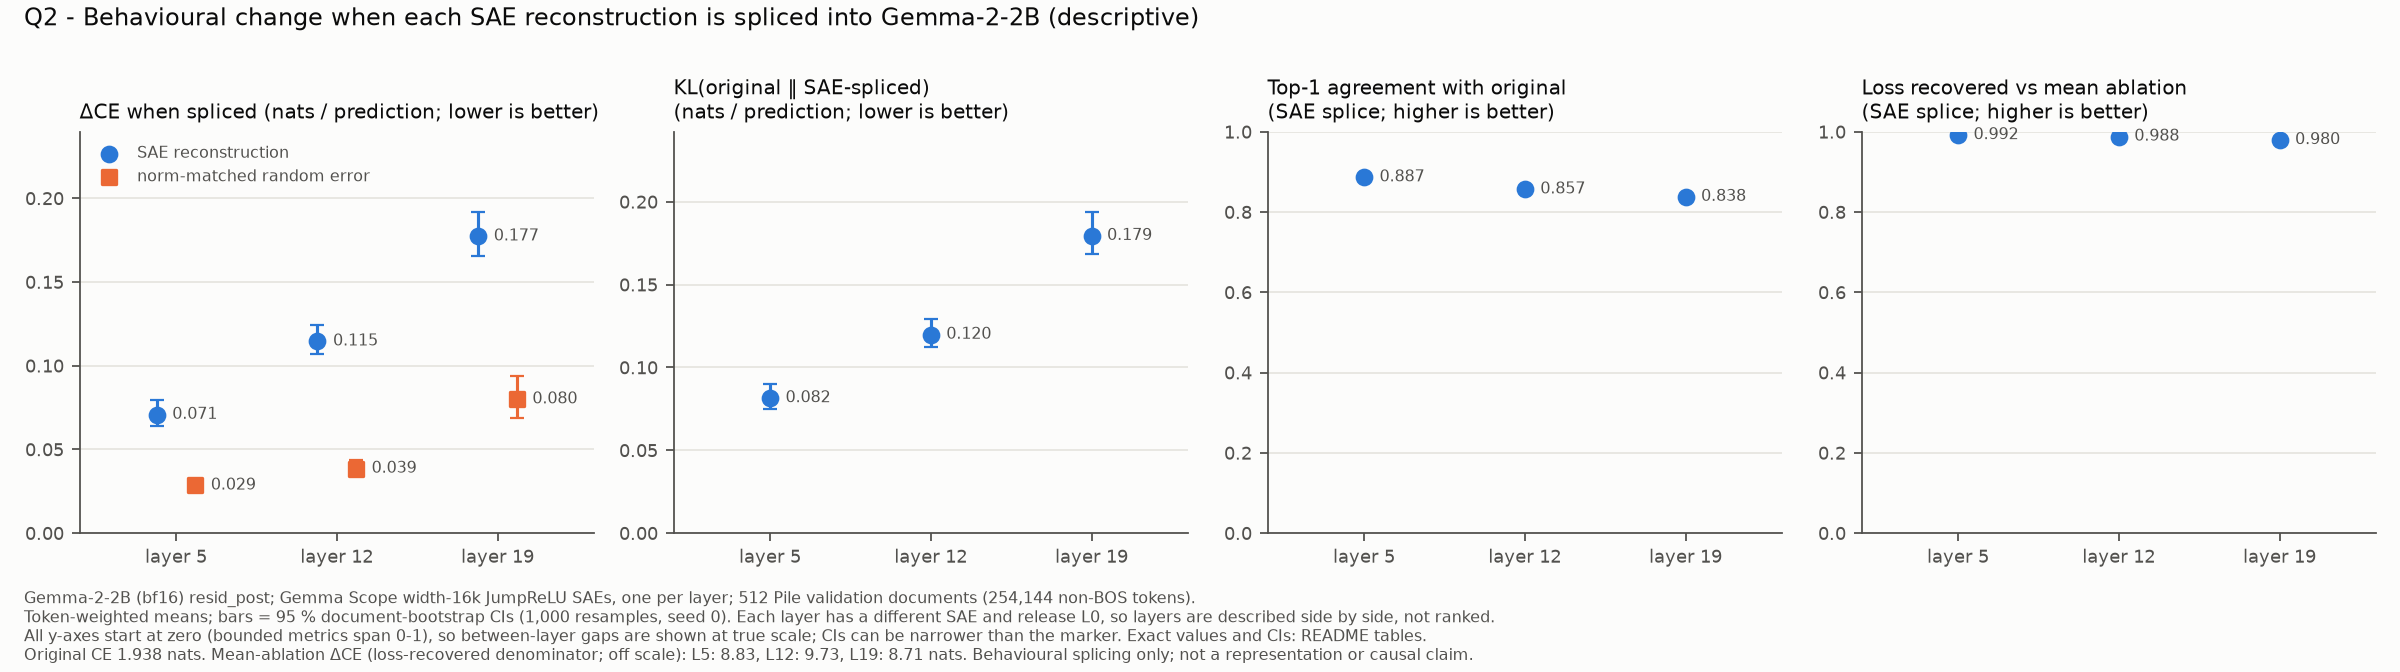
\includegraphics[width=\linewidth]{fig2_splicing_by_layer}
  \caption{M6 behavioural splicing in Gemma-2-2B (\evlabel{validation}): $\Delta$CE for the SAE splice and the
  norm-matched random-error control, KL from the original distribution, top-1 agreement and loss recovered, with 95\,\%
  document-bootstrap intervals. Layers are described side by side, not ranked. Source:
  \texttt{results/\allowbreak{}gemma2\_pile/\allowbreak{}gemma\_scope\_splicing/\allowbreak{}summary\_by\_layer.csv}.}
  \label{fig:m6-splice}
\end{figure}

\section{Evidence Status and Provenance}\label{app:provenance}

Table~\ref{tab:evidence} lists every experiment, its faithfulness level, its evidence label and its result folder.
Code, configurations, pre-registrations and result files are in the repository
\texttt{Fall2026group4/\allowbreak{}fall-2026-group4}. Tables and GPT-2 figures in this paper are generated by
\texttt{scripts/\allowbreak{}shared/\allowbreak{}build\_paper\_artifacts.py} from the committed result files; the Gemma
figures are generated by \texttt{scripts/\allowbreak{}gemma/\allowbreak{}04\_pile\_gemma\_scope\_figures.py}. SAE checkpoints
are listed with SHA-256 hashes in \texttt{docs/\allowbreak{}checkpoint\_registry.csv}. GPT-2 experiments used PyTorch,
TransformerLens \citep{transformerlens2022} and SAELens \citep{saelens2024} on one NVIDIA A10G.

% hand-written evidence-status and provenance table (no numbers; labels from docs/results_registry.md and result READMEs)
\begin{table}[ht]
\centering
\small
\caption{Evidence status and provenance of every experiment used in this paper. Paths are relative to
\texttt{results/}. Historical results that are superseded (original length-confounded RepE probes, early steering,
the circular truth-aware objective) are kept in the repository but are not used as evidence.}
\label{tab:evidence}
\begin{adjustbox}{max width=\linewidth}
\begin{tabular}{llll}
\toprule
Experiment & Level & Evidence label & Result folder \\
\midrule
OWT reconstruction, 108 SAEs & reconstruction & \evlabel{test} & \texttt{openwebtext/reconstruction\_evaluation/uninterrupted\_protocol/} \\
Phase-0 splicing & behaviour & \evlabel{validation} & \texttt{openwebtext/spliced\_evaluation/} \\
M0 within-layer reanalysis & behaviour, information & \evlabel{validation} & \texttt{shared/m0\_within\_layer\_reanalysis/} \\
M1 RepE-LM construction gates & task validity & \evlabel{validation} (train gates) & \texttt{repe/repe\_lm\_gates/} \\
M2 four-level information & information & \evlabel{validation} & \texttt{shared/m2\_four\_level\_faithfulness/} \\
RLM-RP persona preservation & information & \evlabel{validation} & \texttt{repe/repe\_lm\_representation\_preservation/} \\
PCA-CM capacity-matched PCA & information & \evlabel{validation} & \texttt{shared/pca\_capacity\_matched/} \\
M3 causal site sweep & causal (original model) & \evlabel{validation} & \texttt{repe/causal\_site\_sweep/} \\
M4 causal decomposition & causal & \evlabel{validation} & \texttt{repe/sae\_patch\_decomposition/} \\
R5 low-rank causal reference & causal & \evlabel{validation} (descriptive) & \texttt{repe/r5\_causal\_subspace\_skyline/} \\
Method A, IMP-L, output-KL & all levels & \evlabel{validation} & \texttt{geometry\_of\_truth/\{method\_a,e2e\_inspired\}\_layer6/}, \texttt{geometry\_of\_truth/multilayer\_finetune/} \\
E3 causal preservation after fine-tuning & causal & \evlabel{validation} & \texttt{repe/e3\_finetuned\_causal\_preservation/} \\
R2 data-scaled SAEs & all levels & \evlabel{validation}; OWT/GoT \evlabel{confirmed test} & \texttt{openwebtext/r2\_scaled\_saes/} \\
R4 KL fine-tune at fixed L0 & all levels & \evlabel{validation}; OWT/GoT \evlabel{confirmed test} & \texttt{openwebtext/r4\_kl\_finetune/} \\
M5 confirmatory test pass & reconstruction, behaviour, information & \evlabel{confirmed test} & \texttt{shared/m5\_confirmatory\_test/} \\
E2 public \texttt{gpt2-small-res-jb} & information, causal & \evlabel{validation} & \texttt{shared/e2\_public\_sae\_reference/} \\
M6 Gemma Scope on The Pile & reconstruction, behaviour & \evlabel{validation} & \texttt{gemma2\_pile/gemma\_scope\_splicing/} \\
\midrule
E1 task-L0-matched TopK & information, causal & draft pre-registration, not run & \texttt{shared/e1\_task\_l0\_matched\_topk/} \\
SIL mediated SAE-in-the-loop & causal & \evlabel{pre-registered only} & \texttt{repe/sae\_in\_the\_loop\_mediation/} \\
RepE-LM held-out test & information, causal & protocol frozen, no results & \texttt{repe/repe\_lm\_test\_protocol/} \\
PCA-CM test confirmation & information & \evlabel{pre-registered only} & \texttt{shared/pca\_capacity\_matched\_test\_protocol/} \\
R3 Gemma Scope width $\times$ L0 & reconstruction, behaviour & \evlabel{pre-registered only} (separate PR) & not merged \\
\bottomrule
\end{tabular}
\end{adjustbox}
\end{table}


\section{Project History and Corrections}\label{app:history}

Several corrections shaped the final design, and we report them because each changed a conclusion. An early
architecture summary averaged runs with unmatched sparsity; it was replaced by the $\pm10\,\%$ L0 matching rule. Early
``SAE steering'' never placed an SAE in the forward pass and was reclassified. The truth-aware fine-tuning objective was
circular and was replaced by a design with separate teacher and evaluation groups. The original persona prompts were
length-confounded and were replaced by RepE-LM. Correlations pooled across layers were replaced by within-layer
analyses (M0), and frozen-probe failures were re-analysed with noise and PCA references (M2). The original project
proposal asked whether SAE features are causally faithful to their automatically generated labels; the scope was
narrowed to the four-level question of this paper after instructor reviews and internal audits. Historical results,
including the original RepE probes and steering, the layer-6 causal test with 200 controls, an honesty-preservation
fine-tune, feature clamps and Gemma truth-direction steering, are kept in the repository with their status labels and are
not used as evidence here.
